\documentclass[10pt]{beamer}
\setbeameroption{hide notes}
\usepackage{qcircuit}
\usepackage{braket}
\usepackage{tikz}
\usepackage[normalem]{ulem}
% \setbeameroption{show notes on second screen}
\usetheme[sectionpage=progressbar,numbering=counter,block=fill]{metropolis} % Use metropolis theme
\title{Qubits and Quantum Computers}
\date{}
\author{QuTe - Copenhagen}
\institute{Erasmus+}
\logo{
\begin{tikzpicture}[overlay,remember picture]
  \coordinate (logo) at ([xshift=.0cm,yshift=.0cm]current page.south west);
  \node [anchor=south west] at (logo) {
\includegraphics[width=2cm]{img/erasmus_plus.jpg}};
\end{tikzpicture}
}
\titlegraphic{
\begin{tikzpicture}[overlay,remember picture]
  \coordinate (logo) at ([xshift=-.07cm,yshift=-.07cm]current page.south west);
  \node [anchor=south west] at (logo) {
\includegraphics[width=2cm]{img/erasmus_plus.jpg}};
\end{tikzpicture}
}

\begin{document}
\maketitle

\begin{frame}
  \section{Ready, set, go!}
  Grab your \emph{Qubits and Quantum Computers} notes and follow along!
\end{frame}

\begin{frame}
  \section{Bits and Qubits}
\end{frame}

\begin{frame}
  \frametitle{Bits}
  \begin{columns}
    \begin{column}{0.5\linewidth}
      \begin{itemize}
      \item<1-> Two state system
      \item<2-|alert@2> heads or tails
      \item<3-|alert@3> up or down 
      \item<4-|alert@4> charge or no charge
      \item<5-|alert@5> 0 or 1 
      \end{itemize}
    \end{column}
    \begin{column}{0.5\linewidth}
      \centering
      \includegraphics<2>[height=3cm]{img/euro-0.jpg}

      \includegraphics<2>[height=3cm]{img/euro-1.jpg}

      \includegraphics<3>[height=3cm]{img/keep-calm-its-just-a-bit-of-fun.png}
      \includegraphics<3>[height=3cm]{img/keep-calm-its-just-a-bit-of-fun_upside_down.png}

      \includegraphics<4>[height=3cm]{img/ssd.png}

      \only<4>{\footnotemark}

      \onslide<5> \centering \Huge 0 1 
    \end{column}
  \end{columns}
  \only<4>{\footnotetext{Source: \url{https://www.cactus-tech.com/resources/blog/details/solid-state-drive-primer-1-the-basic-nand-flash-cell/}}}
\end{frame}

\begin{frame}
  \frametitle{Bits}
  \begin{block}{Exercise 1 p. 2 in the notes}
    How many possible combinations are possible with 4 bits? Same question but with 10 bits and with \emph{n} bits?
  \end{block}
\end{frame}

\begin{frame}
  \frametitle{A classical computer}
  \Large How many of the numbers are greater than 4?

  \centering 
  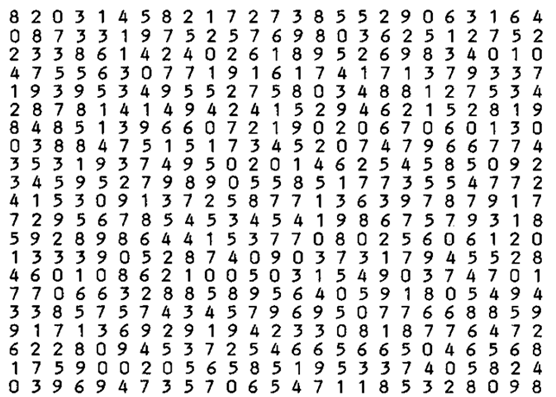
\includegraphics[scale=0.4]{img/random_numbers.png}

  \onslide<2> \normalsize Perfect for a classical computer: One thing at a time, very fast!
  
\end{frame}

\begin{frame}
  \frametitle{Unlock the bike}
  
  \begin{block}{Exercise 2 p. 2 in the notes}
    \begin{columns}
      \begin{column}{0.6\linewidth}
        The code cylinder on a bicycle lock is made up of 5 numbers between 0 and 9: How many possible combinations (i.e. how many codes) does the lock have?
      \end{column}
      \begin{column}{0.3\linewidth}

       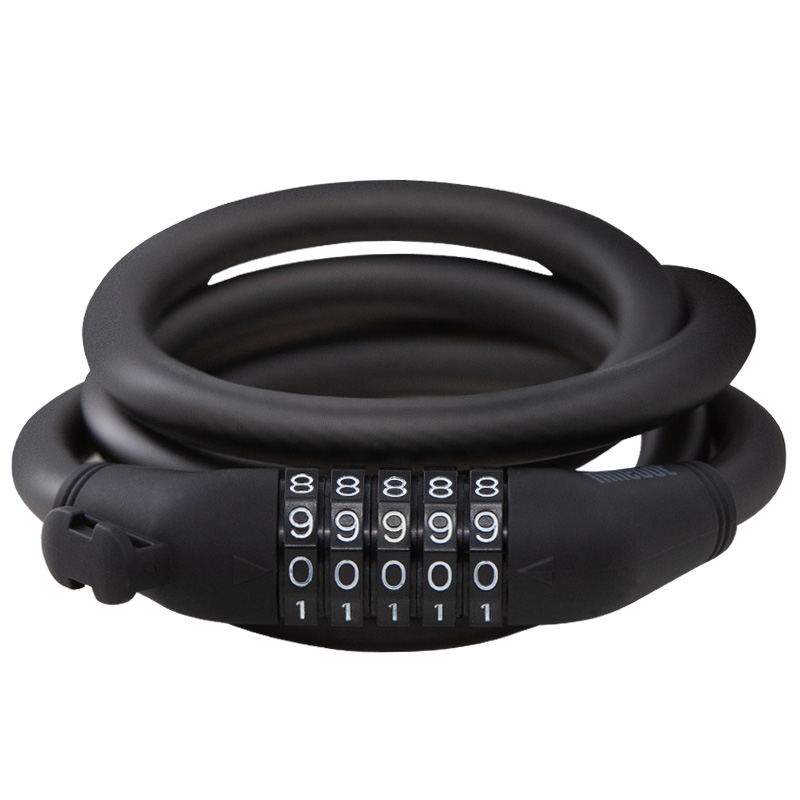
\includegraphics[width=\linewidth]{img/lock5.jpg} 

      \end{column}
    \end{columns}
  \end{block}
\end{frame}

\begin{frame}
  \frametitle{Complexity}
  \begin{columns}
    \begin{column}{0.5\linewidth}
      \begin{block}{Definition 1}
       Complexity of a calculation: the number of operations needed to find a solution to a given problem when the size of the input is \emph{m}. 
      \end{block}
    \end{column}
    \begin{column}{0.5\linewidth}

      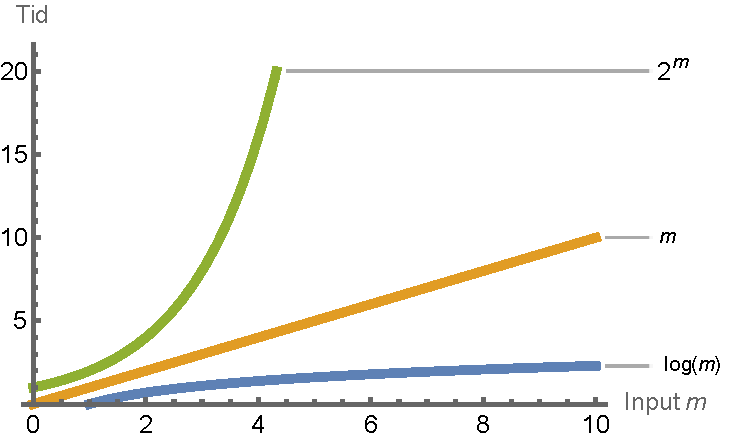
\includegraphics[width=\linewidth]{img/Complexity.pdf}
    \end{column}
  \end{columns}
  \onslide<2> \Large Often the problems increase \emph{exponentially}.
\end{frame}

\begin{frame}
  \frametitle{Exercises}
  \begin{block}{Exercise 3 p. 3 in the notes}
    \begin{columns}
    \begin{column}{0.6\linewidth}
    A classical supercomputer can perform $10^{17}$ operation each second. Vi use it to break a code lock like the one before, except with $m$ digits instead of 5. Assume that the classical supercomputer can check $10^{17}$ different combinations on the lock each second. How large can $m$ be if the classical supercomputer must be able to complete the task in a year?
    \note{Answer is $m=24.5\approx 24$}
    \end{column}
    \begin{column}{0.3\linewidth}

      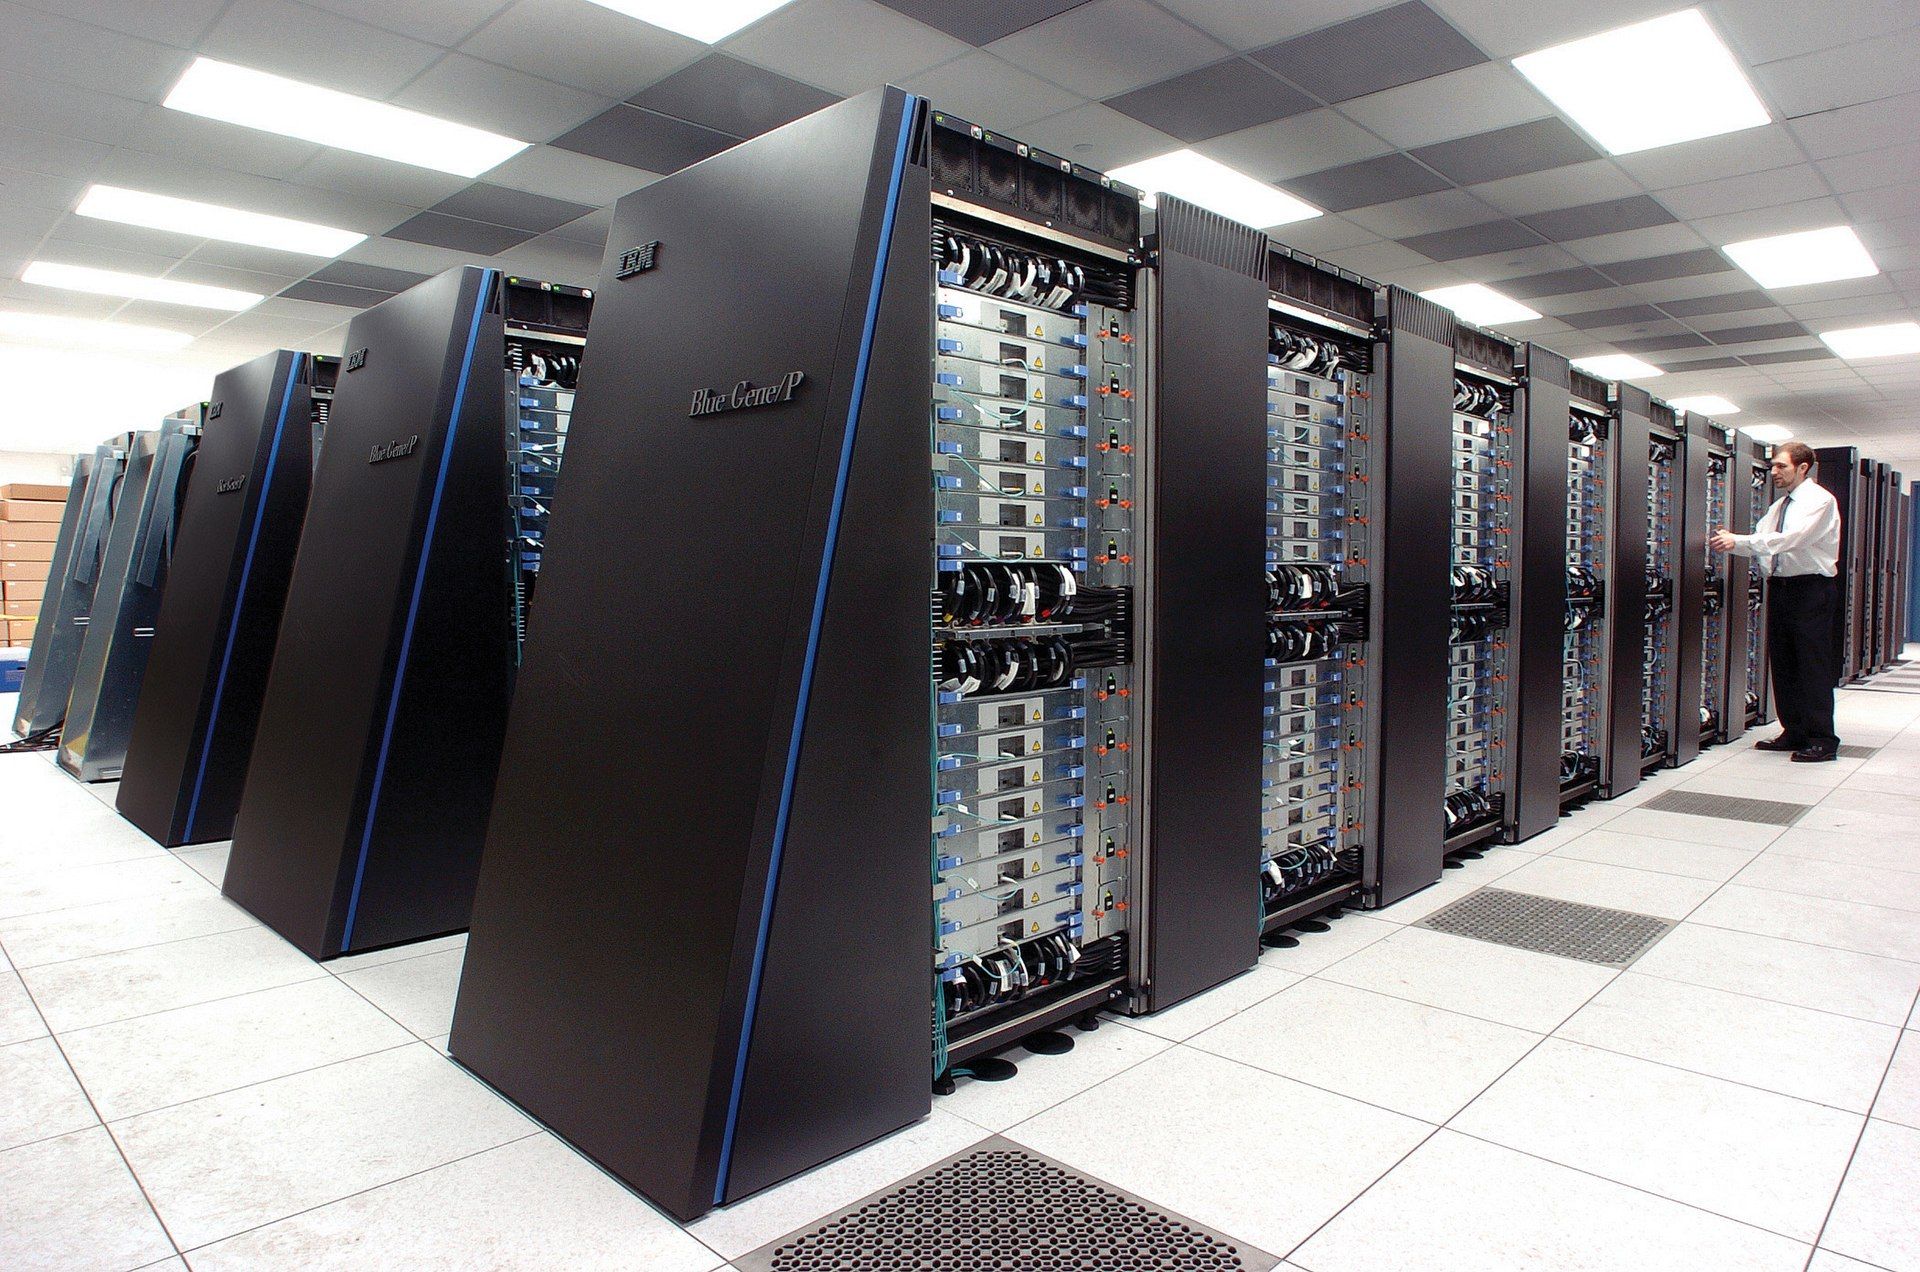
\includegraphics[width=\linewidth]{img/IBM_Blue_Gene_P_supercomputer.jpg}
    \end{column}
    \end{columns}
  \end{block}
  \begin{block}{Exercise 4 p. 3 in the notes}
    \begin{columns}
      \begin{column}{0.6\linewidth}
   Estimate the time it would take you to try all of the possible combinations of the clothes (including accessories!) you choose between each morning. 
      \end{column}
      \begin{column}{0.3\linewidth}
      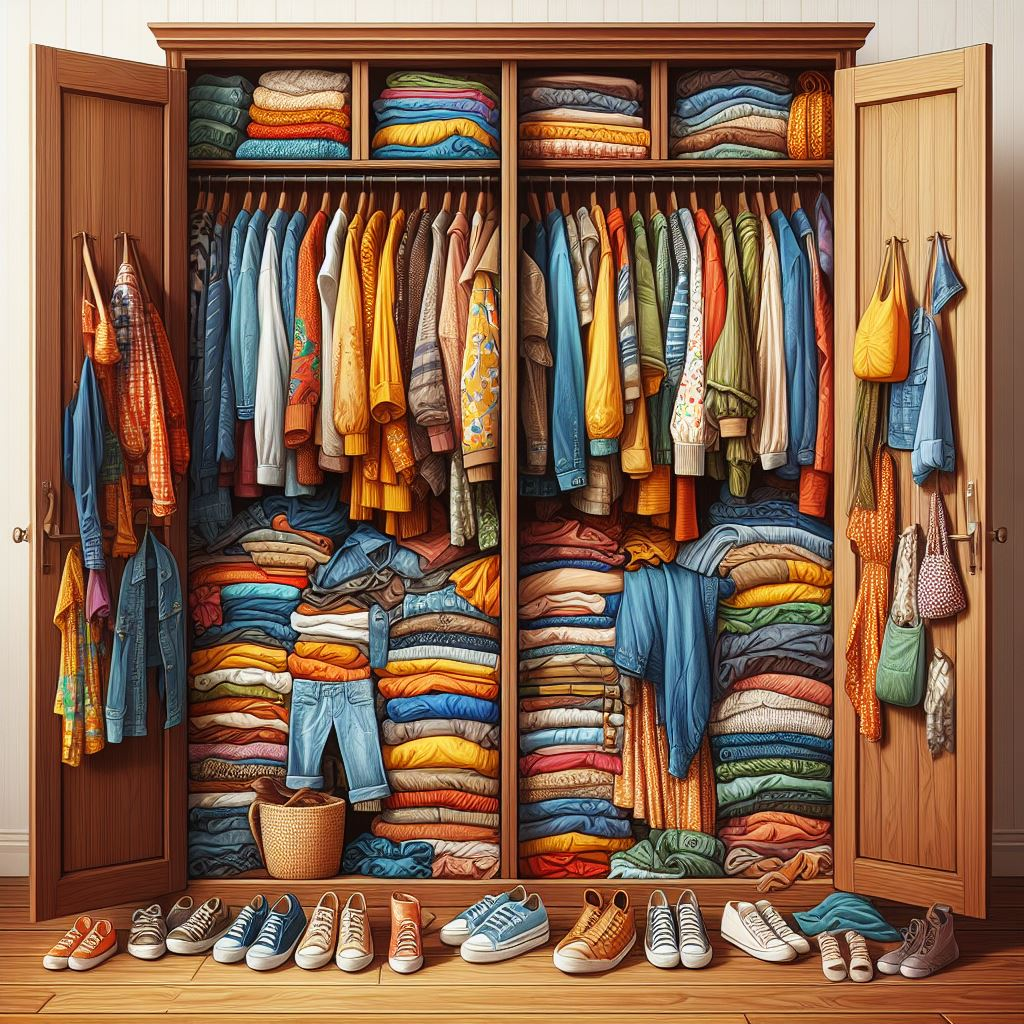
\includegraphics[width=0.8\linewidth]{./img/wardrobe.jpeg}
      \end{column}
    \end{columns}
  \end{block}
\end{frame}
\begin{frame}
  \frametitle{Qubits}
  \begin{columns}
    \begin{column}{0.4\linewidth}
      \begin{itemize}
      \item<+-> Qubits are \emph{quantum systems}.
      \item<2-> Like Bohr's atomic model.
      \item<3-> Qubits are ``simple''. \emph{Only 2 states}.
      \item<4-> You know, ``\textbf{real simple}'', like NV Centers...
      \end{itemize}
    \end{column}
    \begin{column}{0.5\linewidth}
      \centering

      \includegraphics<2-3>[width=6cm]{img/bohrmodel.png}

      \only<2-3>{\footnotemark}

      \includegraphics<4->[width=3cm]{img/nvcenter.png}

      \includegraphics<4->[width=3cm]{img/nvtransitions.png}
    \end{column}
  \end{columns}
  \only<2-3>{\footnotetext{Source: \url{https://www.astronomicalreturns.com/p/section-15-quantum-mechanics.html}}}
\end{frame}

\begin{frame}
  \frametitle{Bits and Qubits}
  \begin{columns}
    \begin{column}{0.5\linewidth}
      \begin{block}{Bits}
        \begin{itemize}
        \item Denoted 0 and 1
        \item If a bit is in state 0 we are sure to measure 0
        \item If a bit is in state 1 we are sure to measure 1
        \item Can \emph{only} be in either state 0 or 1
        \end{itemize}
      \end{block}
    \end{column}
    \begin{column}{0.5\linewidth}
      \begin{block}{Qubits}
        \begin{itemize}
        \item Denoted $\ket{0}$ and $\ket{1}$
        \item If a bit is in state $\ket{0}$ we are sure to measure 0
        \item If a bit is in state $\ket{1}$ we are sure to measure 1
        \item Can be in either state $\ket{0}$, $\ket{1}$ \textbf{or in a superposition of them.}
        \end{itemize}
      \end{block}
    \end{column}
  \end{columns}
  
  \begin{block}<2>{Funny notation}
    A quantum system i described by a state which we denote $\ket{\dots}$.

    The symbol $\ket{\dots}$ is called a \emph{ket}.
  \end{block}
\end{frame}

  \begin{frame}
    \frametitle{Lingual oddities}
    \begin{columns}
      \begin{column}{0.5\linewidth}
        \begin{itemize}
        \item<1-> A ket, $\ket{\dots}$, comes together with a 
        \item<2-> \emph{bra}, $\bra{\dots}$
        \item<3-> Combining them we get a \emph{bra(c)ket}
        \item<4-> or bra(c)ket, $\braket{\dots | \dots}$, like in \emph{parenthesis}
        \end{itemize}
      \end{column}
      \begin{column}{0.4\linewidth}
        \centering
        \includegraphics<2>[width=4cm]{img/bra.jpg}
        \includegraphics<3>[width=4cm]{img/braces.jpg}
        \includegraphics<4->[width=1cm]{img/brackets.png}
      \end{column}
    \end{columns}
  \end{frame}

\begin{frame}
\section{Superposition}
\centering

\includegraphics[width=5cm]{img/superman_clark_kent.jpeg}
\end{frame}

\begin{frame}
  \frametitle{Single Qubit Superposition}
  \begin{columns}
    \begin{column}{0.49\linewidth}
      A single qubit can be in either:
      \begin{itemize}
      \item<1-|alert@2> state $\ket{0}$
      \item<1-|alert@3> state $\ket{1}$
      \item<4-|alert@4> or in a \textbf{superposition} $\ket{\psi}=\alpha \ket{0}+\beta \ket{1}$
      \end{itemize}
    \end{column}
    \begin{column}{0.5\linewidth}

      \includegraphics<2>[width=\linewidth]{img/clark_kent.png}

      \includegraphics<3>[width=\linewidth]{img/superman_new.png}

      \includegraphics<4>[width=\linewidth]{img/superman_clark_kent.jpeg}
    \end{column}
  \end{columns}
\end{frame}

\begin{frame}
  \frametitle{Single Qubit Superposition}
  \begin{columns}
    \begin{column}{0.49\linewidth}
      Or with a coin analogy
      \begin{itemize}
      \item<1-|alert@2> state $\ket{0}$
      \item<1-|alert@3> state $\ket{1}$
      \item<1-|alert@4> or in a \textbf{superposition} $\ket{\psi}=\alpha \ket{0}+\beta \ket{1}$
      \end{itemize}
    \end{column}
    \begin{column}{0.5\linewidth}

      \includegraphics<2>[width=\linewidth]{img/euro-0.jpg}

      \includegraphics<3>[width=\linewidth]{img/euro-1.jpg}

      \includegraphics<4>[width=\linewidth]{img/coin_spinning.jpg}
    \end{column}
  \end{columns}
\end{frame}

\begin{frame}
  \frametitle{Superposition and normalisation}
  \begin{block}{Definition 2: Superposition}
    $\ket{\psi}=\alpha \ket{0}+\beta \ket{1}$

    $\alpha$ and $\beta$ can be choosen arbitrarily as long it is \textbf{normalised}.
  \end{block}
  
  \begin{block}{Definition 3: Normalisation}
    The qubit state $\ket{\psi} = \alpha \ket{0} + \beta \ket{1}$ is normalised if $\alpha^2+\beta^2=1$. 
  \end{block}

  \onslide<2> Read through the example and do exercise 5 and 6 on page 4 in the notes.
\end{frame}

\begin{frame}
  \frametitle{A unit vector}
  \begin{columns}
    \begin{column}{0.5\linewidth}
      You can think of the kets as unit vectors.
      \begin{itemize}
      \item $\ket{0} =
        \begin{pmatrix}
          1 \\0 
        \end{pmatrix}$ Unit vector along x-axis.
      \item $\ket{1} =
        \begin{pmatrix}
         0 \\ 1 
        \end{pmatrix}$ Unit vector along y-axis.
      \item $\ket{\psi}=\alpha \ket{0}+\beta \ket{1}$ Unit vector pointing from (0,0) to $(\alpha , \beta)$ on the unit circle.
      \end{itemize}
    \end{column}
    \begin{column}{0.49\linewidth}
      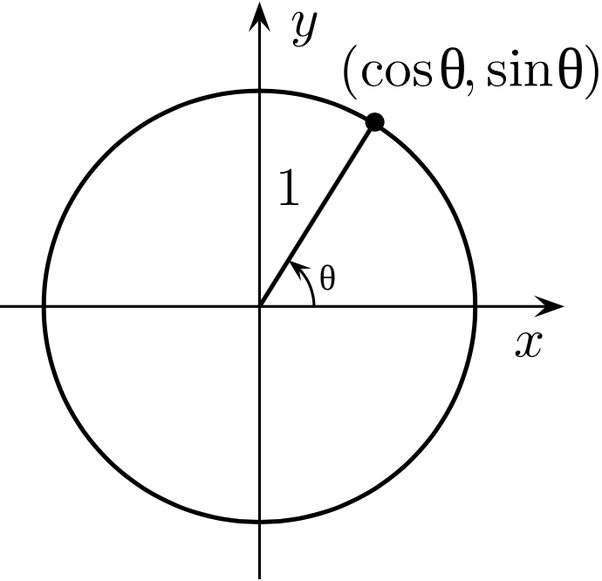
\includegraphics[width=\linewidth]{img/unit-circle.jpg}
    \end{column}
  \end{columns}
  \uncover<2>{\alert{Do exercise 7 on page 4 in the notes.}}
\end{frame}
\begin{frame}
  \section{Measurements and Probabilities}

  \centering
  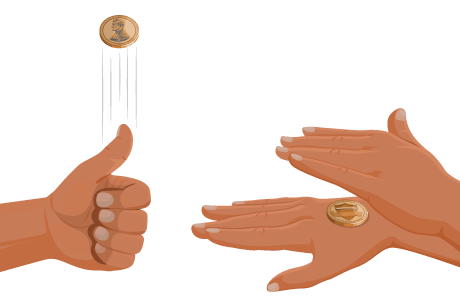
\includegraphics[width=6cm]{img/coin-flip.png}
\end{frame}
\begin{frame}
  \frametitle{Measuring on $\ket{\psi}=\ket{0}$}
  \begin{columns}
    \begin{column}{0.4\linewidth}
      \begin{itemize}
      \item<1-|alert@1> If the qubit is in the state $\ket{\psi}=\ket{0}$.
      \item<2-|alert@2> and the quantum computer performs a measurement.
      \item<3-|alert@3> we get 0 with 100\% probability.
      \end{itemize}
    \end{column}
    \begin{column}{0.5\linewidth}
      \includegraphics<1>[width=\linewidth]{img/euro-0.jpg}
      \includegraphics<2>[width=\linewidth]{img/coin-measure.png}
      \includegraphics<3>[width=\linewidth]{img/euro-0.jpg}
    \end{column}
  \end{columns}
\end{frame}

\begin{frame}
  \frametitle{Measuring on $\ket{\psi}=\ket{1}$}
  \begin{columns}
    \begin{column}{0.4\linewidth}
      \begin{itemize}
      \item<1-|alert@1> If the qubit is in the state $\ket{\psi}=\ket{1}$.
      \item<2-|alert@2> and the quantum computer performs a measurement.
      \item<3-|alert@3> we get 1 with 100\% probability.
      \end{itemize}
    \end{column}
    \begin{column}{0.5\linewidth}
      \includegraphics<1>[width=\linewidth]{img/euro-1.jpg}
      \includegraphics<2>[width=\linewidth]{img/coin-measure.png}
      \includegraphics<3>[width=\linewidth]{img/euro-1.jpg}
    \end{column}
  \end{columns}
\end{frame}

\begin{frame}
  \frametitle{Measuring $\ket{\psi}=\alpha \ket{0}+\beta \ket{1}$}
  \begin{columns}
    \begin{column}{0.4\linewidth}
      \begin{itemize}
      \item<1-|alert@1> If the qubit now is in the state $\ket{\psi}=\alpha \ket{0}+\beta \ket{1}$.
      \item<2-|alert@2> and the quantum computer performs a measurement.
      \item<3-|alert@3> we get \textbf{either} 0 or 1 and \textbf{never} something in between.
      \item<4-|alert@4> We cannot predict the outcome. Only calculate the probabilities!
      \item<5-|alert@5> We have to abandon \textbf{determinism}.
      \end{itemize}
    \end{column}
    \begin{column}{0.5\linewidth}
      \centering

      \includegraphics<1>[width=\linewidth]{img/coin_spinning.jpg}

      \includegraphics<2>[width=\linewidth]{img/coin-measure.png}

      \includegraphics<3->[width=3cm]{img/euro-0.jpg}

      \onslide<3-> \Huge or \\

      \includegraphics<3->[width=3cm]{img/euro-1.jpg}
    \end{column}
  \end{columns}
\end{frame}

\begin{frame}
  \frametitle{Probabilities}
  \begin{block}{Definition 4: Probability}
    If  our qubit is in the state $|\psi\rangle$ then the probability of measuring 0 is given by $P_0 = (\langle0|\psi\rangle)^2$ and the probability of measuring 1 is given by $P_1 = (\langle1|\psi\rangle)^2$.
  \end{block}
  \begin{block}{Definition 5: Rules}
    \begin{equation*}\label{regneregler}
    \braket{0|0}=\braket{1|1}=1 \quad {\rm and} \quad 
        \braket{0|1}=\braket{1|0}=0
    \end{equation*}
  \end{block}
  \uncover<2->{
 	\begin{itemize}
    \item<2-|alert@2> Remember: We have defined $\ket{0}=\begin{pmatrix} 1\\0 \end{pmatrix}$ and $\ket{1}=\begin{pmatrix} 0\\1 \end{pmatrix}$. Therefore we can interpret $\braket{a|b}$ as the \textit{dot product} of the vectors $a$ and $b$. \\
	\item<3-|alert@3> Show the rules by calculating the dot product of all combinations of $\ket{0}$ and $\ket{1}$.
	\end{itemize}}  

\end{frame}
\begin{frame}
  \frametitle{Time to work}
  Read through the examples, remarks and do the exercises on page 7 and 8 in the notes.

  \uncover<2->{
    When you are done, you should realise that:
    
    \begin{block}{Definition 6: Alternative to definition 4}
      Probability: If our qubit is in the state $\ket{\psi}=\alpha \ket{0}+\beta \ket{1}$ then the probability of measuring 0 is given by $P_0=\alpha^2$ and the probability of measuring 1 by $P_1=\beta^2$.
    \end{block}
  }
\end{frame}

\begin{frame}
  \frametitle{Collapse of the state}
  \begin{columns}
    \begin{column}{0.5\linewidth}
      \begin{itemize}
      \item<1-> A qubit is initially in a superposition state $\ket{\psi}$.
      \item<2-> We do a measurement...
      \item<3-> and get 0.
      \item<4-> We do a new measurement on the same qubit in its current state...
      \item<5-> and get 0.
      \item<6-|alert@6> The initial state is collapsed.
      \end{itemize}
    \end{column}
    \begin{column}{0.5\linewidth}
            \includegraphics<1>[width=\linewidth]{img/coin_spinning.jpg}
            \includegraphics<2>[width=\linewidth]{img/coin-measure.png}
            \includegraphics<3>[width=\linewidth]{img/euro-0.jpg}
            \includegraphics<4>[width=\linewidth]{img/coin-measure.png}
            \includegraphics<5->[width=\linewidth]{img/euro-0.jpg}
    \end{column}
  \end{columns}
      \begin{block}{Definition 7}<7>
        \footnotesize
        If we measure and the result is 0, then the state of the qubit immediately after the measurement is the state $\ket{0}$. Likewise, if the measurement result is 1, then the state of the qubits immediately after the measurement is the state $\ket{1}$.
      \end{block}
\end{frame}
\begin{frame}
  \frametitle{The measurement affects the state}
  \begin{columns}
    \begin{column}{0.5\linewidth}
      \footnotesize
      \begin{itemize}
      \item<1-> A qubit is in the state $\ket{\psi}$ (superposition).
      \item<2-> We do a measurement...
      \item<3-> and get 0.
        
      \item<4-> We do the same all over again on \emph{another} (identical) qubit in the same state $\ket{\psi}$ (superposition).
      \item<5-> We do a measurement...
      \item<6-> and get 1.
      \item<7-|alert@7> What can we say about the probabilities?
      \item<8-|alert@8> Only that the probabilities $P_0$ and $P_1$ are non zero!
      \item<9-|alert@9> What can we do to determine the probabilities?
      \item<10-|alert@10> Take a huge amount of identical states...
      % \item<12-|alert@12> and perform the same measurement again and again.
      % \item<13-|alert@13> Now we have a distribution and can predict the probabilities.
      \end{itemize}
    \end{column}
    \begin{column}{0.5\linewidth}
      \footnotesize
      \begin{itemize}
      \item<11-|alert@11> and perform the same measurement on each of them.
      \item<12-|alert@12> Now we have a distribution and can predict the probabilities.
        \end{itemize}
            \includegraphics<1>[width=\linewidth]{img/coin_spinning.jpg}
            \includegraphics<2>[width=\linewidth]{img/coin-measure.png}
            \includegraphics<3>[width=\linewidth]{img/euro-0.jpg}
            \includegraphics<4>[width=\linewidth]{img/coin_spinning.jpg}
            \includegraphics<5>[width=\linewidth]{img/coin-measure.png}
            \includegraphics<6->[width=\linewidth]{img/euro-1.jpg}
    \end{column}
  \end{columns}
\end{frame}

  \begin{frame}
    \frametitle{Time for some exercise}
    Do exercise 10 on page 8 in the notes.

    \begin{block}{Exercise 10}
      Show that the state $\frac{1}{5}(3\ket{0}+4\ket{1})$ is normalised and determine the probability, $P_1$, of measuring 1 if the qubit is initially in the state $\ket{\psi}=\frac{1}{5}(3\ket{0}+4\ket{1})$.
    \end{block}
  \end{frame}

\begin{frame}
  \section{Operators and Diagrams}
\end{frame}

\begin{frame}
  \frametitle{Single Qubit operators}
  We want to do something with the qubits! We do that with \textbf{operators}.
  \begin{block}{Definition 9: Operator}
    An operator acts on a state and returns a state.
  \end{block}
\end{frame}

\begin{frame}
  \frametitle{Doing nothing}
  \centerline{\Qcircuit @C=2em @R=1.5em {\lstick{\ket{0}}   &    \qw &    \rstick{\ket{0}} \qw}}
  \vfill
  \begin{itemize}
  \item A single qubit is drawn as a horizontal line. 
  \item Each end indicate the state of the qubit.
  \item Read from left to right.
  \end{itemize}
  \vfill
\end{frame}
  
\begin{frame}
  \frametitle{The Z operator}
  \begin{block}{Definition 10: The operator Z}
    $Z= \ket{0}\bra{0}-\ket{1}\bra{1}$
  \end{block}
    \centerline{
\Qcircuit @C=2em @R=1.5em {
   \lstick{\ket{0}}   &   \gate{Z}   &    \rstick{\ket{0}} \qw \\
   \lstick{\ket{1}}   &   \gate{Z}   &    \rstick{-\ket{1}} \qw \\
}
}
\begin{itemize}
\item<2-> An operator acts on a state from the \emph{left}.
\item<3->  i.e. $Z \ket{\psi} = \left(\ket{0}\bra{0}-\ket{1}\bra{1}\right) \ket{\psi}$
  
\item<4-|alert@4> What does $Z$ do?
\end{itemize}
\begin{block}{Exercise 15 in the notes.}<4->
  Use the definition of $Z$, i.e. that $Z=|0\rangle\langle0|-|1\rangle\langle1|$, and let it act on $\ket{0}$ and $\ket{1}$. Show that the result is the same as depicted in the figure.
\end{block}
\end{frame}
\begin{frame}
  \frametitle{The X operator}
  \begin{block}{Definition 11: The operator X}
    $X = \ket{1}\bra{0}+\ket{0}\bra{1}$
  \end{block}
\centerline{
\Qcircuit @C=2em @R=1.5em {
   \lstick{\ket{0}}   &   \gate{X}   &    \rstick{\ket{1}} \qw \\
   \lstick{\ket{1}}   &   \gate{X}   &    \rstick{\ket{0}} \qw \\
}
}
\onslide<2-> What does the X operator do?
\begin{block}{Exercise 16 in the notes.}<2->
  Show what happen when $X$ acts on the state $\frac{1}{\sqrt{2}}(|0\rangle+|1\rangle)$. If you have studied Appendix 2, then note that you have just shown that $\frac{1}{\sqrt{2}}(|0\rangle+|1\rangle)$ is an eigenstate of $X$ with eigenvalue 1!
\end{block}
\end{frame}

\begin{frame}
  \frametitle{The Hadamard operator, $H$}
  \begin{block}{Definition 12: The operator $H$}
    $H = \frac{1}{\sqrt{2}}\left( \ket{0}\bra{0}+ \ket{0}\bra{1} +\ket{1}\bra{0}-\ket{1}\bra{1} \right)$
  \end{block}	\centerline{
	\Qcircuit @C=1em @R=.7em {
   \lstick{\ket{0}}   & \qw & \gate{H} & \qw & \qw & \rstick{\frac{1}{\sqrt{2}}(\ket{0}+\ket{1})}  \\
   \lstick{\ket{1}}   & \qw & \gate{H} & \qw & \qw & \rstick{\frac{1}{\sqrt{2}}(\ket{0}-\ket{1})}  
}
}
\begin{itemize}
\item<2-|alert@2> Work through the exercises 17, 18, 19 on page 14 and 15 in the notes. Consult the surrounding examples if in doubt or if you need a hint.
\end{itemize}
\end{frame}

\begin{frame}
  \frametitle{Diagrams with measurements}
  \centerline{
\scalebox{1.0}{
\Qcircuit @C=1.0em @R=0.2em @!R { \\
	 	\nghost{{q} :  } & \lstick{{q} : \  \ket{0}} & \gate{\mathrm{X}} % \barrier[0em]{0} 
		& \qw & \meter & \qw & \qw\\
	 	\nghost{\mathrm{{c} :  }} & \lstick{\mathrm{{c} : \ \ \ \ \ \, }} &% \lstick{/_{_{1}}} 
		\cw & \cw & \dstick{_{_{\hspace{0.0em}0}}} \cw \ar @{<=} [-1,0] & \cw & \cw\\
 }}}
\begin{enumerate}
\item<2-> q for \textbf{q}ubit and c for \textbf{c}lassical bit.
\item<3-> qubit starts in state $\ket{0}$
\item<4-> Operator $X$ acts on the state.
\item<5-> The new state is measured (acted on by the measuring operator)
\item<6-> The outcome of the measurement is stored in classical bit number 0 (counting from 0 instead of 1).
\item<7-> The diagram before the measurement translates to the following calculation: $$X \ket{0} = \left(\ket{1}\bra{0} + \ket{0}\bra{1}  \right)\ket{0}$$
\item<8-|alert@8> Predict the outcome of the measurement.
\end{enumerate}
\end{frame}

\begin{frame}
  \frametitle{Example and exercise}
  Read through the example concerning the Hadamard operator starting at the bottom of 16 continuing to page 17 in the notes.
  Then do exercise 21 on page 17 in the notes.

  \begin{block}{Exercise 21}
   \centerline{
\scalebox{1.0}{
\Qcircuit @C=1.0em @R=0.2em @!R { \\
	 	\nghost{{q} :  } & \lstick{{q} : \  \ket{0}  } & \gate{\mathrm{H}} & \gate{\mathrm{Z}}  %\barrier[0em]{0}
		 & \qw & \meter & \qw & \qw\\
	 	\nghost{\mathrm{{c} :  }} & \lstick{\mathrm{{c} :  \ \ \ \ \ \,  }} & % \lstick{/_{_{1}}} 
		\cw & \cw & \cw & \dstick{_{_{\hspace{0.0em}0}}} \cw \ar @{<=} [-1,0] & \cw & \cw\\
\\ }}
} 

Our qubit start out in the state $\ket{0}$. Explain what the state of our qubit is after $H$ and then $Z$ have acted on it, i.e. calculate $ZH\ket{0}$. Then determine what the probability is of measurement giving 0 and 1, respectively.
  \end{block}
\end{frame}
\begin{frame}
  \frametitle{And now for something completely different}
  \centering
  
\includegraphics[width=6cm]{img/completely_different.jpeg}
\end{frame}
\begin{frame}
  \frametitle{And now for something completely \sout{different} related \footnote{Google is your friend :)}}
  \centering
  
\includegraphics[width=6cm]{img/completely_different.jpeg}
\end{frame}
\begin{frame}
  \section{IBM Q}
  \centering
  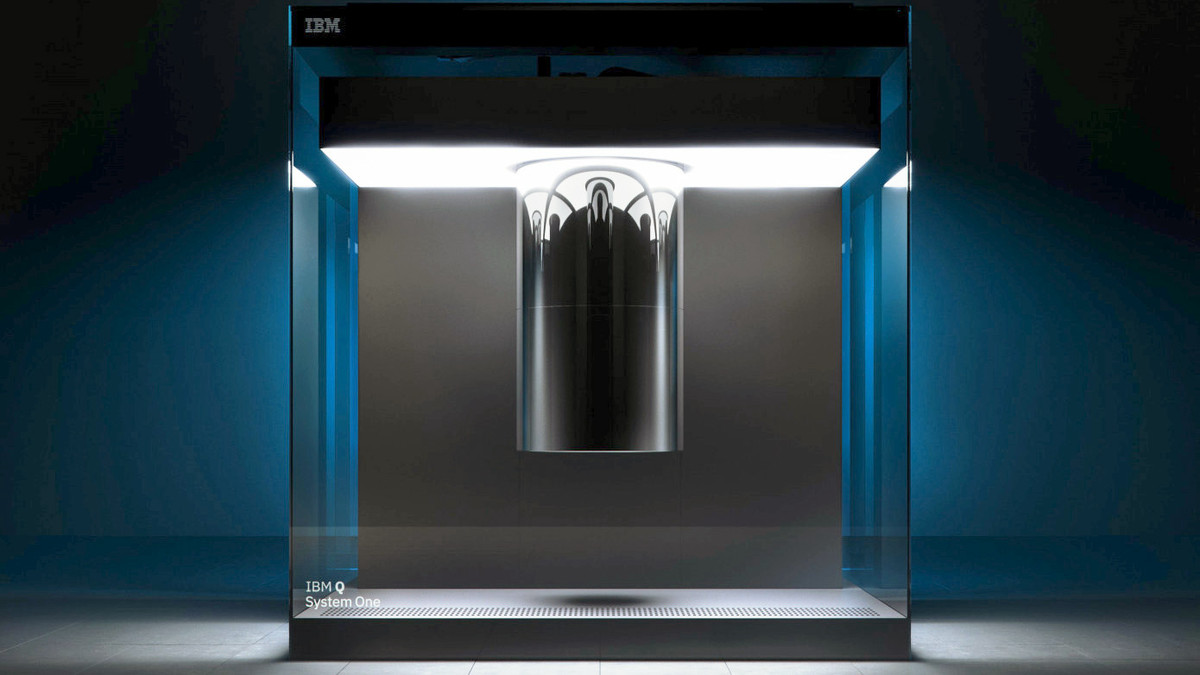
\includegraphics[width=0.7\linewidth]{img/IBMQ.jpg}
\end{frame}

\begin{frame}
  \frametitle{Access IBM Q}
  \begin{itemize}
  \item Visit \href{https://quantum-computing.ibm.com/}{https://quantum-computing.ibm.com/}
  \item Create an IBM account or sign in with one of the other options.
  \item Go to ``Lab''.
  \end{itemize}
  \centering
  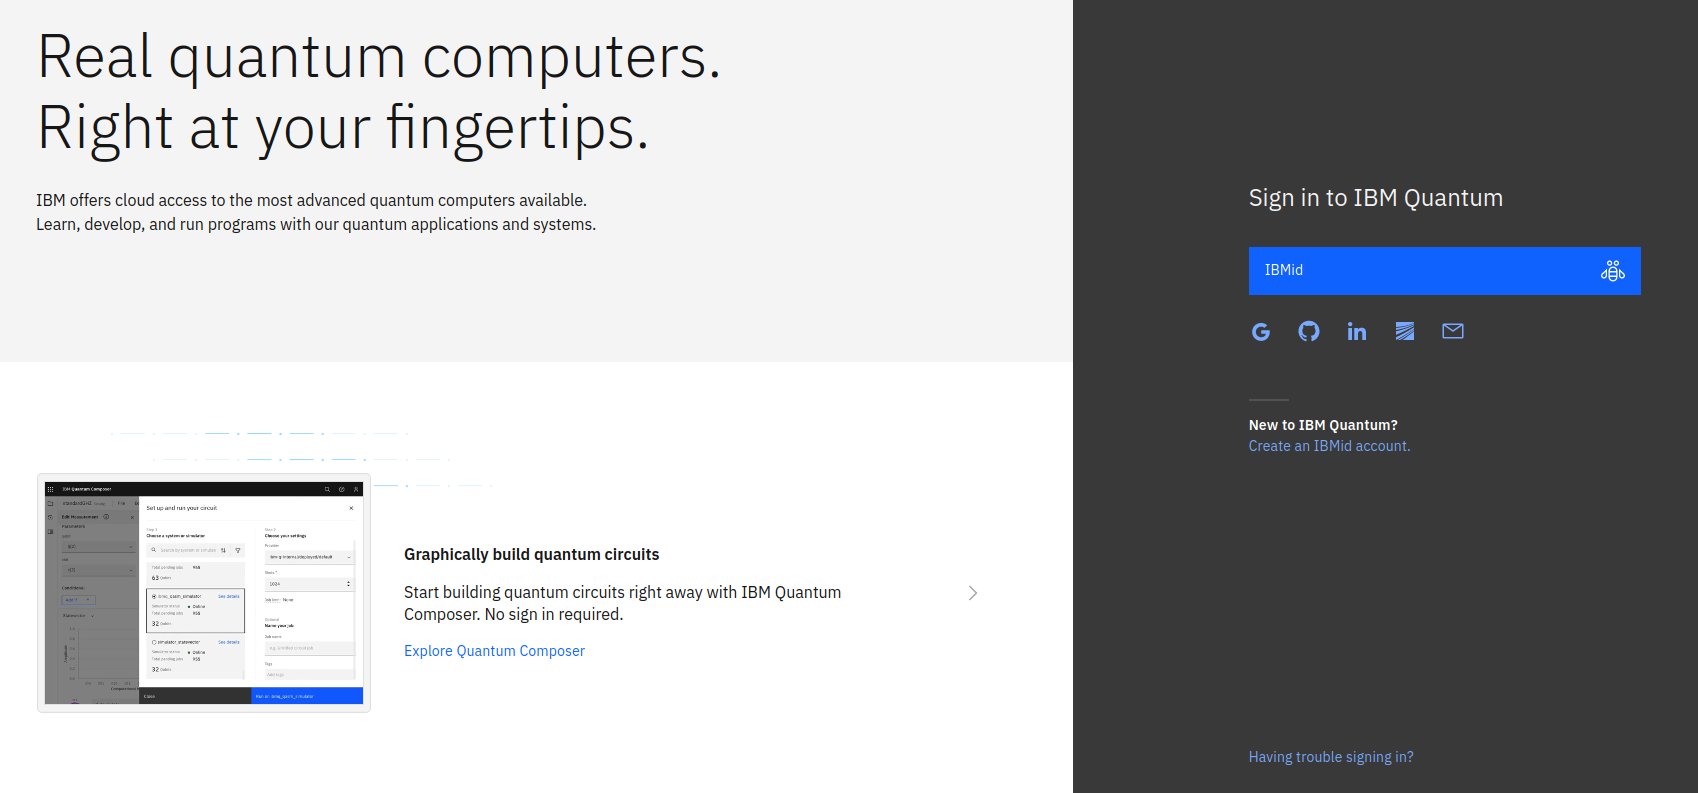
\includegraphics[width=9cm]{img/ibmq-login.png}
\end{frame}

\begin{frame}
  \frametitle{Upload the IBM Q exercises}
  Upload the following exercises to the lab file browser. (You can use drag and drop).
  \begin{itemize}
  \item MeasurementSingleQubit.ipynb
  \item MeasurementTwoQubits.ipynb
  \item MeasurementEntangledQubits.ipynb
  \item GroversAlgorithm.ipynb
  \end{itemize}

  \centering
  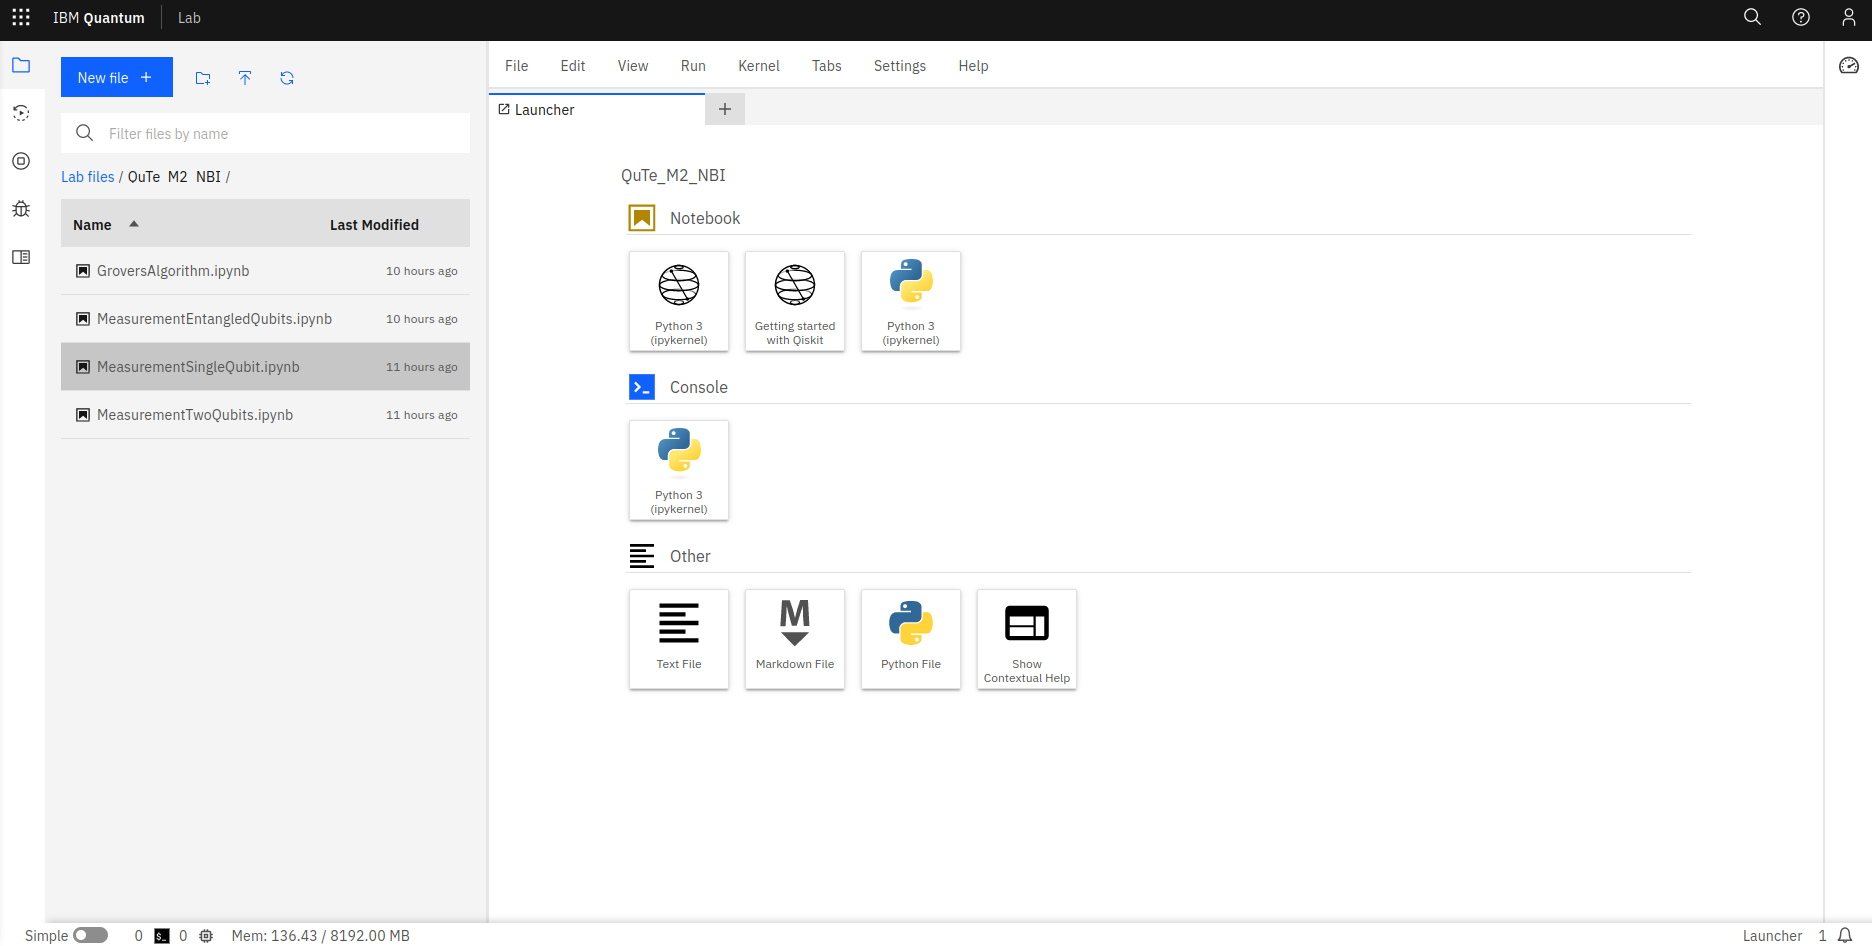
\includegraphics[width=9cm]{img/ibmq-upload.png}
\end{frame}

\begin{frame}
  \frametitle{Single Qubit Measurements}
  Run the \emph{Measurement SingleQubit.ipynb} notebook and follow the instructions. You are now able to perform \textbf{real} work on a real \textbf{quantum computer}! (If you set the variable sym=False)
  \begin{center}
  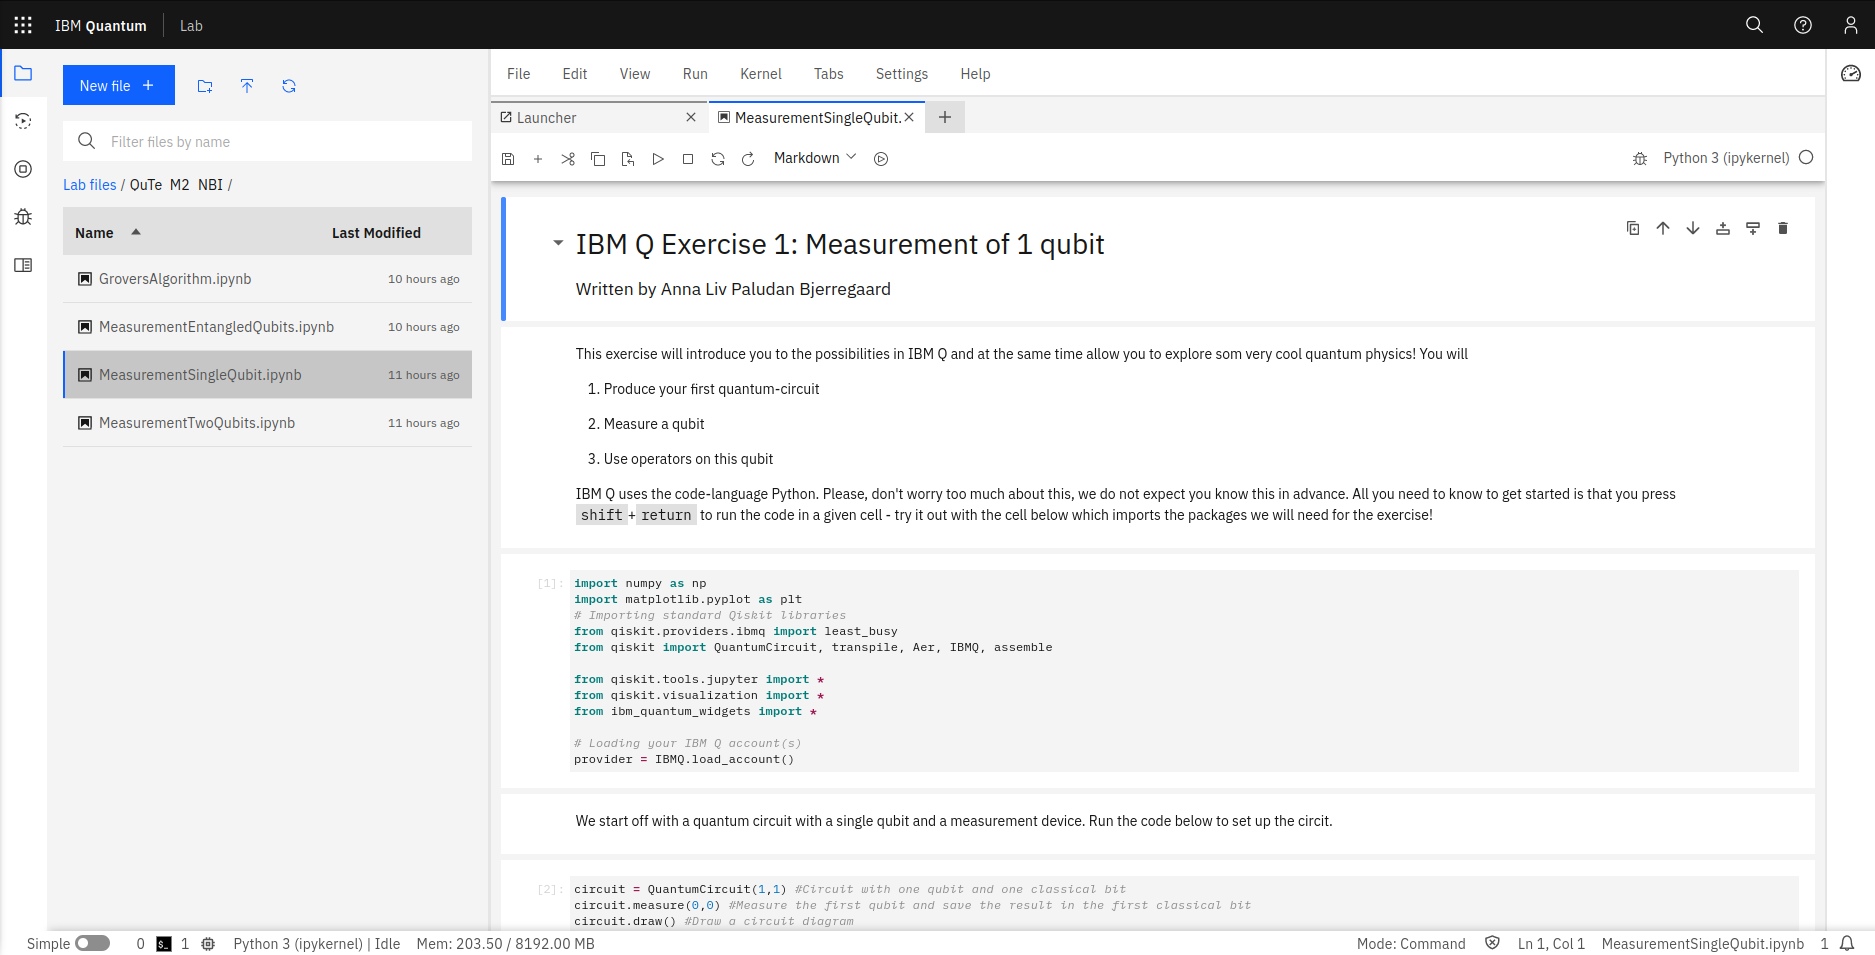
\includegraphics[width=10cm]{img/ibmq-single-qubit.png}
  \end{center}
\end{frame}

\begin{frame}
  \frametitle{Pun intended! Did you get it?}
 \footnotesize Now to something completely \sout{different} related.
  \begin{center}
  
\includegraphics[width=6cm]{img/completely_different.jpeg}
  \end{center}
  \uncover<2->{\footnotesize The quote is from Monty Python $\to$ IBM Q \emph{is} related $\to$ IBM Q uses \emph{Python} $\to$ Python is named after Monty Python, \uncover<3>{\alert{because programming should be fun!}}}
\end{frame}

\begin{frame}
  \frametitle{Back to school!}
  \centering
  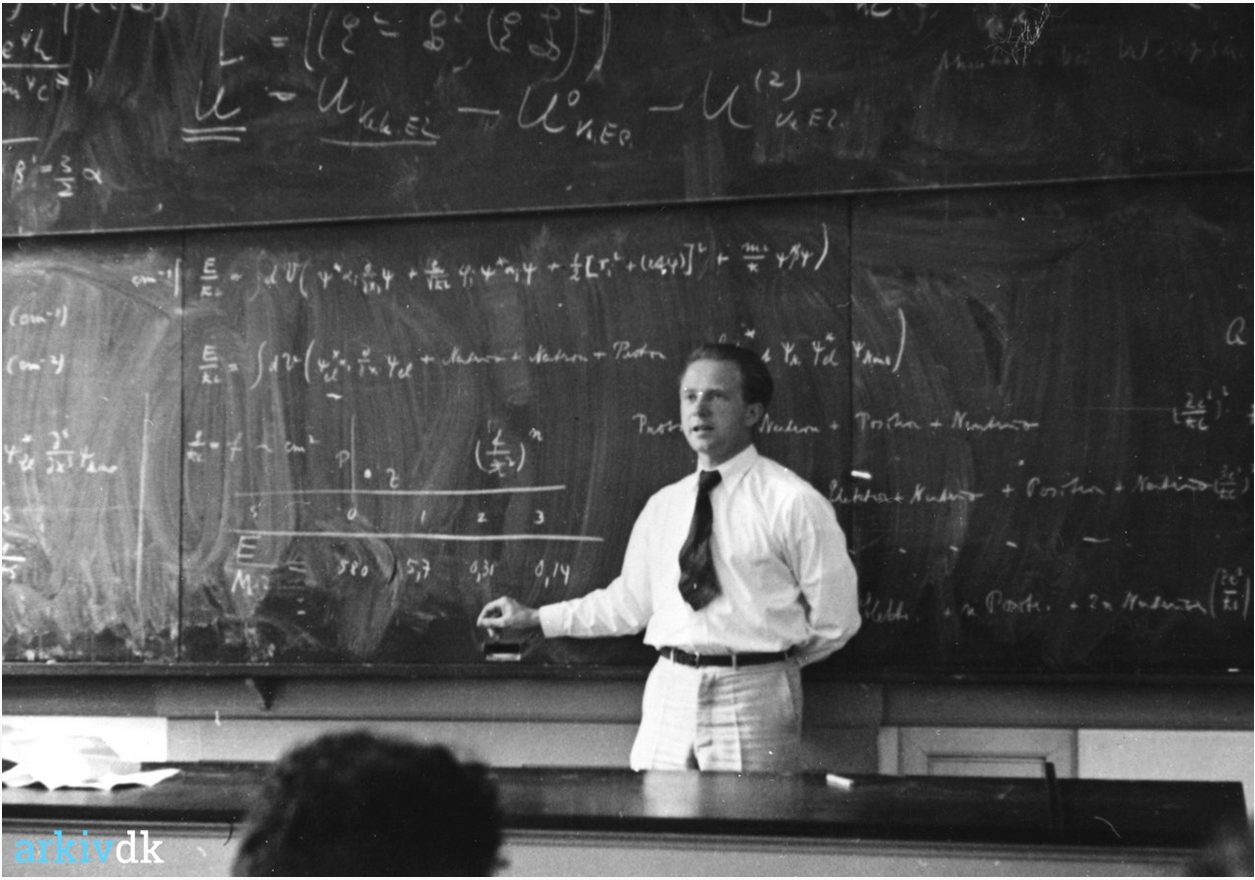
\includegraphics[width=10cm]{img/back-to-school.png}
\end{frame}
\begin{frame}
  \frametitle{One,\sout{two,} too Many}
  How many is \emph{many?}
  \begin{itemize}
  \item<2->\only<2>{One} \only<3>{One, two} \only<4>{One, two, many} \only<5->{\sout{One, two, many}}
  \end{itemize}
  \onslide<6->{This time it is only}
  \begin{itemize}
  \item<7-> \only<7>{One} \only<8->{One, many}
  \end{itemize}
  \onslide<9->{This time around we are going to work with \textbf{two} qubit systems.}

  \onslide<10-> {With two or more qubits we can do...}
\end{frame}

\begin{frame}
  \section{Entanglement}
  \centering
  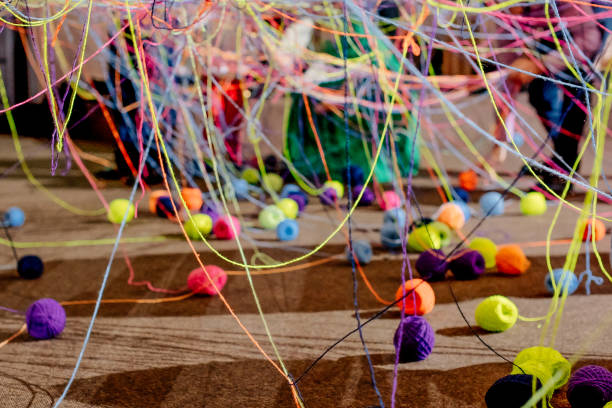
\includegraphics[width=0.7\linewidth]{img/tangled-yarn.jpg}
\end{frame}

\begin{frame}
  \frametitle{Two qubit entanglement}
  \begin{block}{Definition 8: Entanglement}
  Two qubits are entangled if the state of one qubit depends on the other. When two qubits are entangled it is \textit{impossible} to write the total state as a product of a state of the first qubits and a state of the second.
  \end{block}
  \uncover<2>{Let us see some examples. (Read the examples in Chapter V section 10 in the notes, page 10 and 11)}
\end{frame}

\begin{frame}
  \frametitle{None entangled two qubit systems}
  \begin{block}{Two qubits not entangled}
    If qubit 1 is in the state $\ket{0}$ and qubit 2 is in the state $\ket{1}$, then the total state of the qubits is $\ket{1}\ket{0} = \ket{10}$
  \end{block}
  \begin{block}{Another two qubits not entangled}
    If the state of qubit 1 is $\ket{0}$ and the state of qubit 2 is $\frac{1}{\sqrt{2}}\left( \ket{0}+\ket{1} \right)$, then the total state of the two qubits is $\frac{1}{\sqrt{2}}\left( \ket{0}+\ket{1} \right)\ket{0}=\frac{1}{\sqrt{2}}\left( \ket{00}+\ket{10} \right)$.
  \end{block}

  \begin{block}{A third example}
    Two \emph{not entangled} qubits: The two qubits in the state $\frac{1}{5}\left( 3 \ket{01}+4 \ket{11} \right)$ are not entangled, since we can write the state as $\frac{1}{5}\left( 3 \ket{01}+4 \ket{11} \right)= \frac{1}{5}\left( 3 \ket{0}+4 \ket{1} \right)\ket{1}$.
  \end{block}
\end{frame}

\begin{frame}
  \frametitle{Entangled two qubit systems}
  \begin{block}{Example: Entangled qubits}
    Two qubits are in the state $\frac{1}{\sqrt{2}}\left( \ket{10}+\ket{01} \right)$. They are \emph{entangled} because the state of the first qubit depends on the state of the second: If the first qubit is 1 then the other is 0, and vice versa (if the first qubit is 0 then the second i 1). To put it differently, you can not write the total state $\frac{1}{\sqrt{2}}\left( \ket{10}+\ket{01} \right)$ as a product of two states $\ket{\dots}\ket{\dots}$.
  \end{block}

  \begin{block}{Another example}
    The two qubits in the state $\frac{1}{5}\left( 3\ket{00}+4 \ket{11} \right)$ are entangled.
  \end{block}
\end{frame}

\begin{frame}
  \frametitle{Time for some exercise}
  \centering
  % 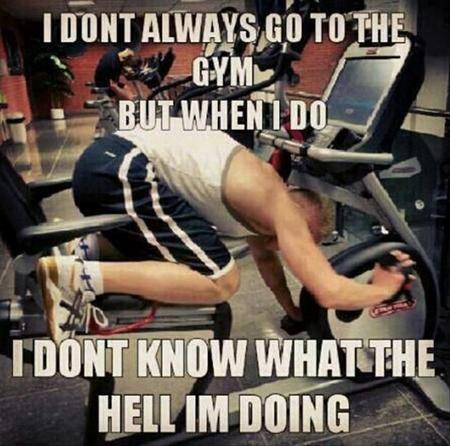
\includegraphics[width=7cm]{img/exercise-meme.jpg}
  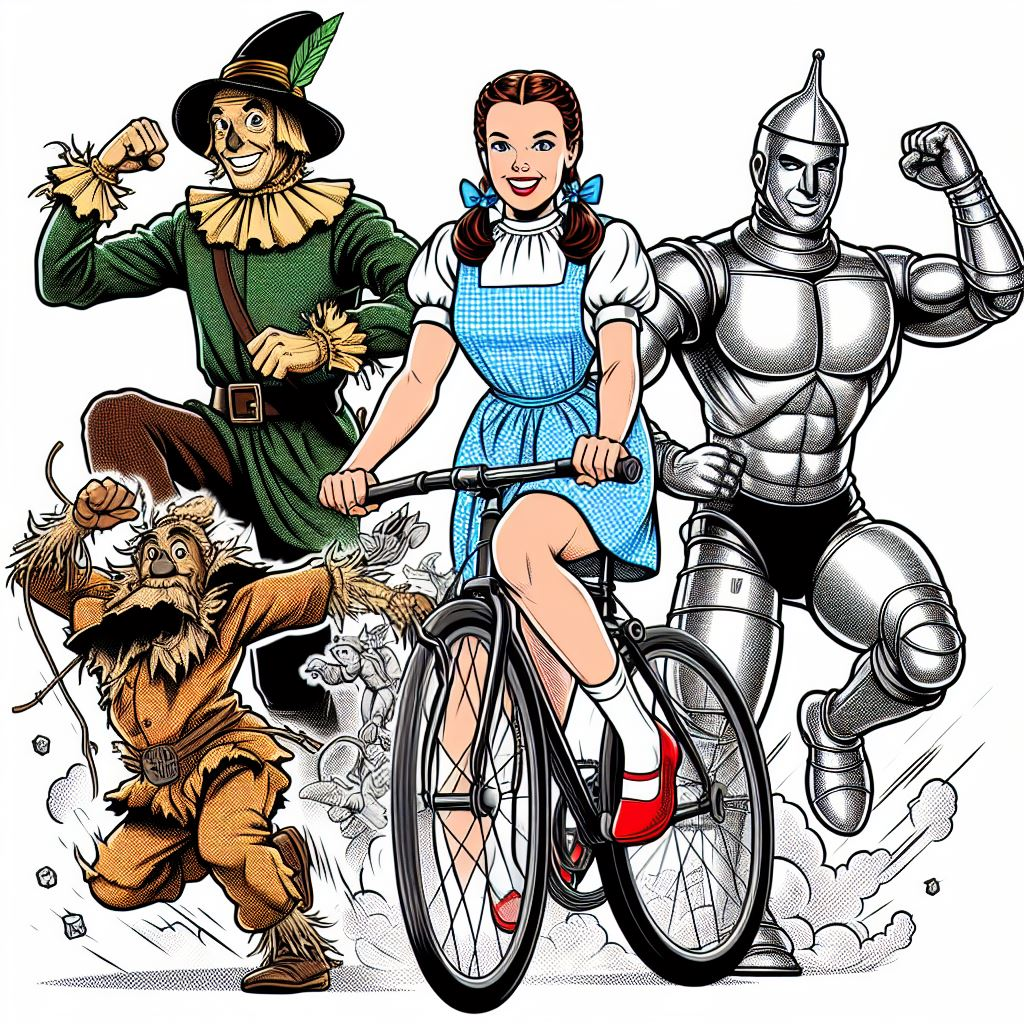
\includegraphics[width=7cm]{img/exercise.jpeg}
\end{frame}

\begin{frame}
  \frametitle{Exercises}
  \begin{block}{Exercise 11 page 10 in the notes.}
    Two qubits are in the state $\ket{01}$. What is the state of  qubit 1? what about qubit 2?
  \end{block}
  \begin{block}{Exercise 12 page 11 in the notes.}
    Determine which of the following two-qubit states are entangled: 
         \begin{enumerate}
             \item $\ket{11}$
             \item $\frac{1}{\sqrt{2}}(\ket{11}+\ket{00})$
             \item $\frac{1}{\sqrt{2}}(\ket{10}+\ket{11})$ 
         \end{enumerate}
  \end{block}
\end{frame}

\begin{frame}
 \section{But what is the difference between entangled and none entangled states?}
 \onslide<2>{\centering It's all about the measurements.}
\end{frame}

\begin{frame}
  \frametitle{None entangled qubits}
  \centering
      Two qubits are in the state $\ket{01}$(read from the right).
  \begin{columns}
    \begin{column}{0.5\linewidth}
      \begin{itemize}
      \item Qubit 2 is in state $\ket{0}$ .
      \end{itemize}
      \begin{center}
        \includegraphics<1>[height=3cm]{img/euro-0.jpg}
        \includegraphics<2>[height=3cm]{img/coin-measure.png}
        \includegraphics<3->[height=3cm]{img/euro-0.jpg}
        \end{center}
    \end{column}
    \begin{column}{0.5\linewidth}
      \begin{itemize}
      \item Qubit 1 is in state $\ket{1}$.
      \end{itemize}
      \begin{center}
        \includegraphics<1>[height=3cm]{img/euro-1.jpg}
        \includegraphics<2>[height=3cm]{img/coin-measure.png}
        \includegraphics<3->[height=3cm]{img/euro-1.jpg}
        \end{center}
    \end{column}
  \end{columns}
  \visible<1>{$\phantom{a}$}%
  \only<2>{Measuring on any of the qubits}%
  \only<3>{does not alter the other.}%
  \only<4->{The state remains unaltered.}
\end{frame}

\begin{frame}
  \frametitle{Entangled qubits}
  \centering
      Two qubits are in the entangled state $\frac{1}{\sqrt{2}}\left( \ket{01} + \ket{10} \right)$.
  \begin{columns}
    \begin{column}{0.5\linewidth}
      \begin{center}
        Qubit 2

        \includegraphics<1-2>[height=3cm]{img/coin_spinning.jpg}
        \includegraphics<3->[height=3cm]{img/euro-1.jpg}
        \end{center}
    \end{column}
    \begin{column}{0.5\linewidth}
      \begin{center}
        Qubit 1

        \includegraphics<1>[height=3cm]{img/coin_spinning.jpg}
        \includegraphics<2>[height=3cm]{img/coin-measure.png}
        \includegraphics<3->[height=3cm]{img/euro-0.jpg}
        \end{center}
    \end{column}
  \end{columns}
  \visible<1>{$\phantom{a}$}%
  \only<2>{We measure qubit 1.}%
  \only<3>{and get 0.}%
  \only<4>{Qubit 1 is now in state $\ket{0}$ forcing the total state to be $\ket{10}$}%
  \only<5>{The measurement on qubit 1 affects qubit 2 instantaneously.}
\end{frame}
\begin{frame}
  \frametitle{Albert Einstein}
    \centering
  \begin{quote}
    I cannot seriously believe in it because the theory cannot be reconciled with the idea that physics should represent a reality in time and space, free from \textbf{spooky action at a distance}.
    \end{quote}
    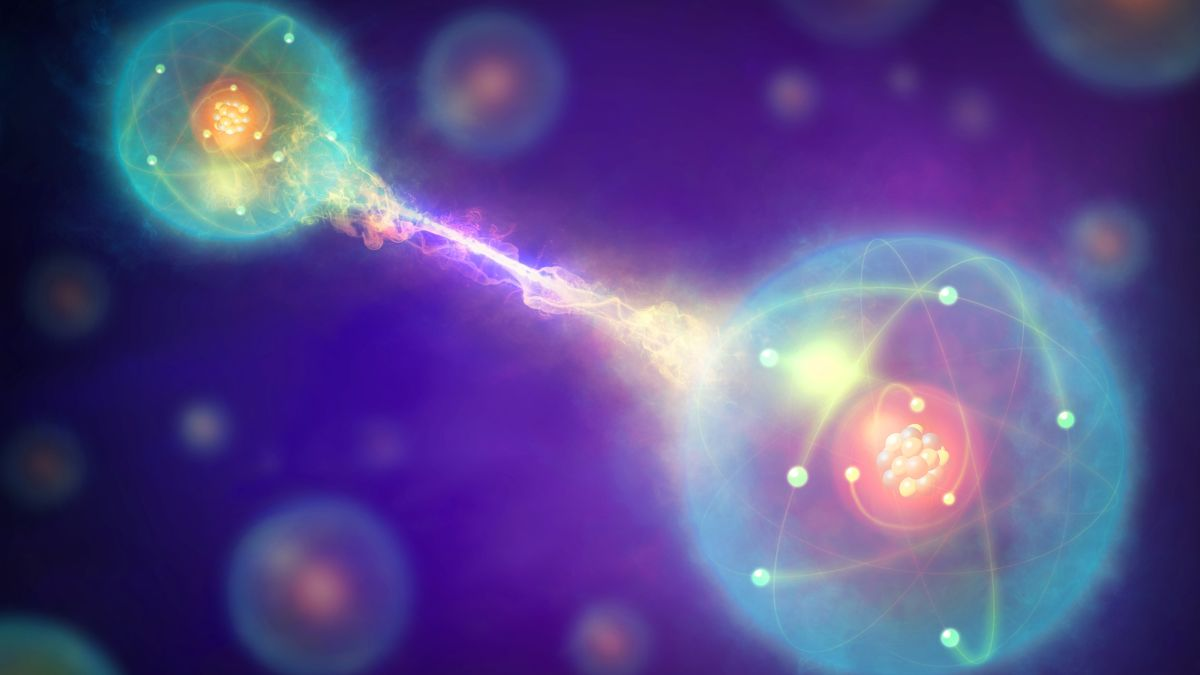
\includegraphics[width=6cm]{img/entanglement.jpg}
\end{frame}

\begin{frame}
  \frametitle{Untangle these exercises}
  \begin{block}{Exercise 13 page 11 in the notes.}
    Two qubits are in the state $\frac{1}{\sqrt{2}}(\ket{00}+\ket{11})$. What is the probability of a measurement on the first qubit giving 0 and 1, respectively. If we measure the first qubit, and the outcome is 1, what is the total state of the two qubits immediately after the measurement?
  \end{block}
  \begin{block}{Exercise 14 page 12 in the notes.}
   Two qubits are in the state $\frac{1}{5}(3\ket{01}-4\ket{10}$. Will a measurement on the second qubit affect the state of the first qubit? 
  \end{block}
\end{frame}
\begin{frame}
  \section{Operating on two qubits}
  \centering
  The Controlled NOT gate
\end{frame}
\begin{frame}
  \frametitle{The CNOT gate}
  \begin{block}{Definition 13: The CNOT operator}
    First qubit is the control bit
 $  \ \ \ \ CNOT=\ket{00}\bra{00}+\ket{11}\bra{01}+\ket{10}\bra{10}+\ket{01}\bra{11}$
 \\ Second qubit is the control bit $ \ CNOT=\ket{00}\bra{00}+\ket{01}\bra{01}+\ket{11}\bra{10}+\ket{10}\bra{11}$
  \end{block}
  \uncover<2->{But what does it do?}

  \uncover<3->{If the control qubit is 0, it does nothing.}

  \uncover<4->{If the control qubit is 1, it changes the state of the other qubit (by applying the $X$ operator in the other qubit.)}
\end{frame}
\begin{frame}
  \frametitle{Let us check}
  \begin{block}{Example: $CNOT\ket{01}$ with first qubit as control}
    
\begin{align*}
  CNOT \ket{01} &=\left( \ket{00}\bra{00}+\ket{11}\bra{01}+\ket{10}\bra{10}+\ket{01}\bra{11} \right) \ket{01} \\
                &= \ket{00}\braket{00|01}+\ket{11}\braket{01|01}+\ket{10}\braket{10|01}+\ket{01}\braket{11|01} \\
                &= \ket{00} 0 + \ket{11} 1 + \ket{10} 0 + \ket{10} 0 \\
  &= \ket{11}
\end{align*}
  \end{block}
  As you can see the first qubit remains unchanged while the second qubit changes from state $\ket{0}$ to $\ket{1}$.

  \uncover<2->{\alert{Do a quick check of the other combinations of $CNOT$ and the states $\ket{00}, \ket{01},\ket{10},\ket{11}$.}}
\end{frame}

\begin{frame}
  \frametitle{Creating an entangled state}
  \begin{block}{Example: $CNOT$ on $\frac{1}{\sqrt{2}}\left( \ket{01}+\ket{00} \right)$ with qubit 1 as control}
    
    \scriptsize
\begin{align*}
  CNOT \frac{1}{\sqrt{2}}\left( \ket{01}+\ket{00} \right) &= \left( \ket{00}\bra{00}+\ket{11}\bra{01}+\ket{10}\bra{10}+\ket{01}\bra{11} \right)\frac{1}{\sqrt{2}}\left( \ket{01}+\ket{00} \right) \\
  &= \frac{1}{\sqrt{2}}\left( \ket{11} + \ket{00} \right)
\end{align*}
    
  \end{block}
  \uncover<2->{\alert{We went from an none entangled state to an entangled state!}}
\end{frame}

\begin{frame}
  \frametitle{Creating an entangled state from scratch}
  \centerline{	 	
	\scalebox{1}{%
\Qcircuit @C=1.4em @R=1.8em {
	  \lstick{\ket{0}} &    \gate{H}     & \ctrl{1} & \qw \\
	  \lstick{\ket{0}} &  \qw   \ & \targ & \qw
        }}}
    The diagram shows how we, using a Hadamard and a $CNOT$-operator, can produce the entangled state $\frac{1}{\sqrt{2}}(|11\rangle+|00\rangle)$. The dot in the $CNOT$-operator indicates the control qubit and the other end, which looks like a sight, points to the qubit which the CNOT operators does something to (the target qubit).
    
    \uncover<2->{The state goes}

    \uncover<2->{from $\ket{0}\ket{0}$}

    \uncover<3->{to $\ket{0}\frac{1}{\sqrt{1}}\left( \ket{0}+\ket{1} \right)=\frac{1}{\sqrt{2}}\left( \ket{00}+\ket{01} \right)$}

    \uncover<4->{to $CNOT \frac{1}{\sqrt{2}}\left( \ket{00}+\ket{01} \right)$}

    \uncover<5->{to the final \emph{entangled} state $\frac{1}{\sqrt{2}}\left( \ket{11}+\ket{00} \right)$}
\end{frame}
\begin{frame}
  \frametitle{Measuring entangled states}
  \centerline{
\scalebox{1.0}{
\Qcircuit @C=1.0em @R=0.2em @!R { \\
	 	\nghost{{q} :  } & \lstick{{q_1} : \  \ket{0}  } & \gate{\mathrm{H}} & \ctrl{1}  %\barrier[0em]{0}
		 & \qw & \meter & \qw &\qw & \qw\\
		 	 	\nghost{{q} :  } & \lstick{{q_2} : \  \ket{0}  } & \qw & \targ  %\barrier[0em]{0}
		 & \qw & \qw & \meter & \qw & \qw\\
	 	\nghost{\mathrm{{c} :  }} & \lstick{\mathrm{{c} :  \ \ \ \ \ \,  }} & % \lstick{/_{_{1}}} 
		\cw & \cw & \cw & \dstick{_{_{\hspace{0.0em}0}}} \cw \ar @{<=} [-2,0] & \dstick{_{_{\hspace{0.0em}1}}} \cw \ar @{<=} [-1,0] & \cw & \cw\\
\\ }}
}
In the figure we perform measurements on each of the two qubits which are in the state $\frac{1}{\sqrt{2}}(|11\rangle+|00\rangle)$ before the measurement.  The measurement on the first qubit will give 0 with $50\%$ probability. If the measurement gives 0, the state of the first qubit is $|0\rangle$ after the measurement. Therefore, the total state of the two qubits is $|00\rangle$ after we have measured 0 for the first qubit. We now measure the second qubit and get 0 with $100\%$ probability, since the second qubit is in the state $|0\rangle$.
\end{frame}

\begin{frame}
  \frametitle{Back to IBM Q}
  \centering
  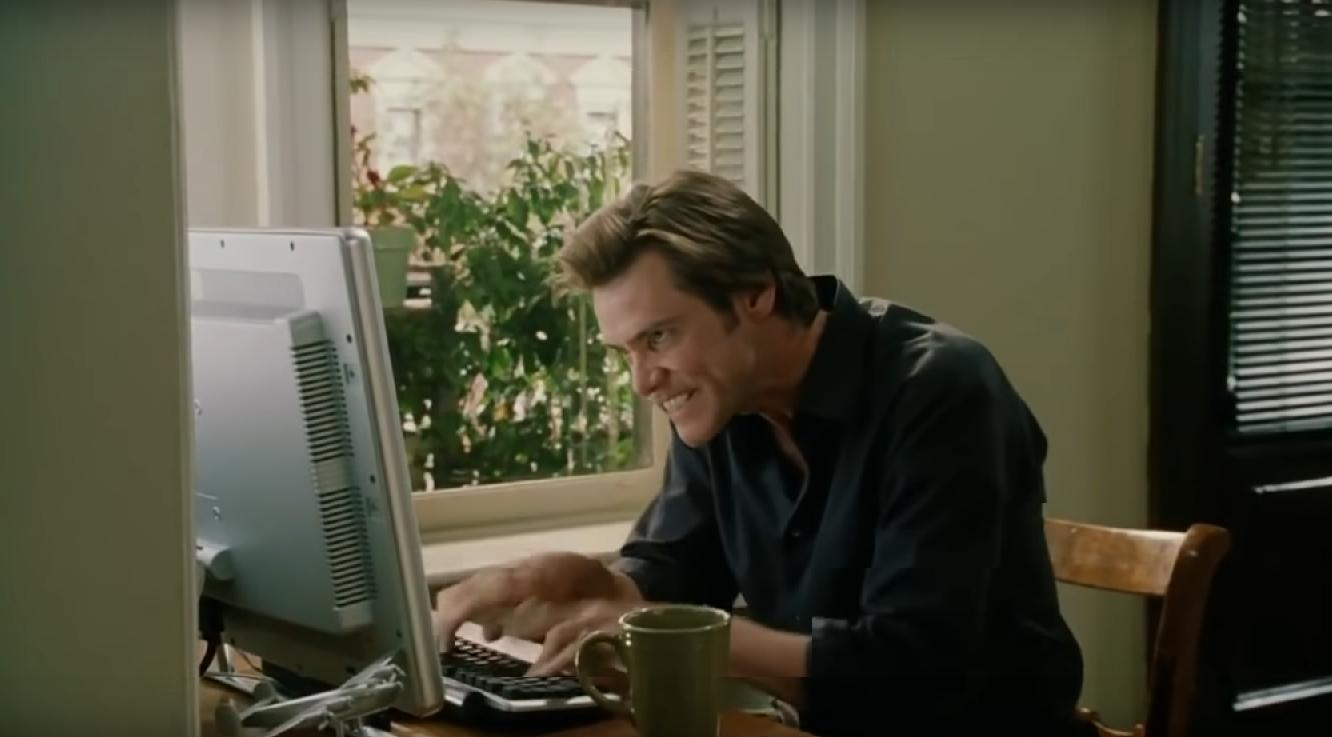
\includegraphics[width=8cm]{img/typing.jpg}
\end{frame}

\begin{frame}
  \frametitle{Measuring two (non-entangled) qubits}
  Log in to \href{https://lab.quantum-computing.ibm.com}{https://lab.quantum-computing.ibm.com} and fire up exercise \emph{MeasurementTwoQubits.pynb}

  \begin{center}
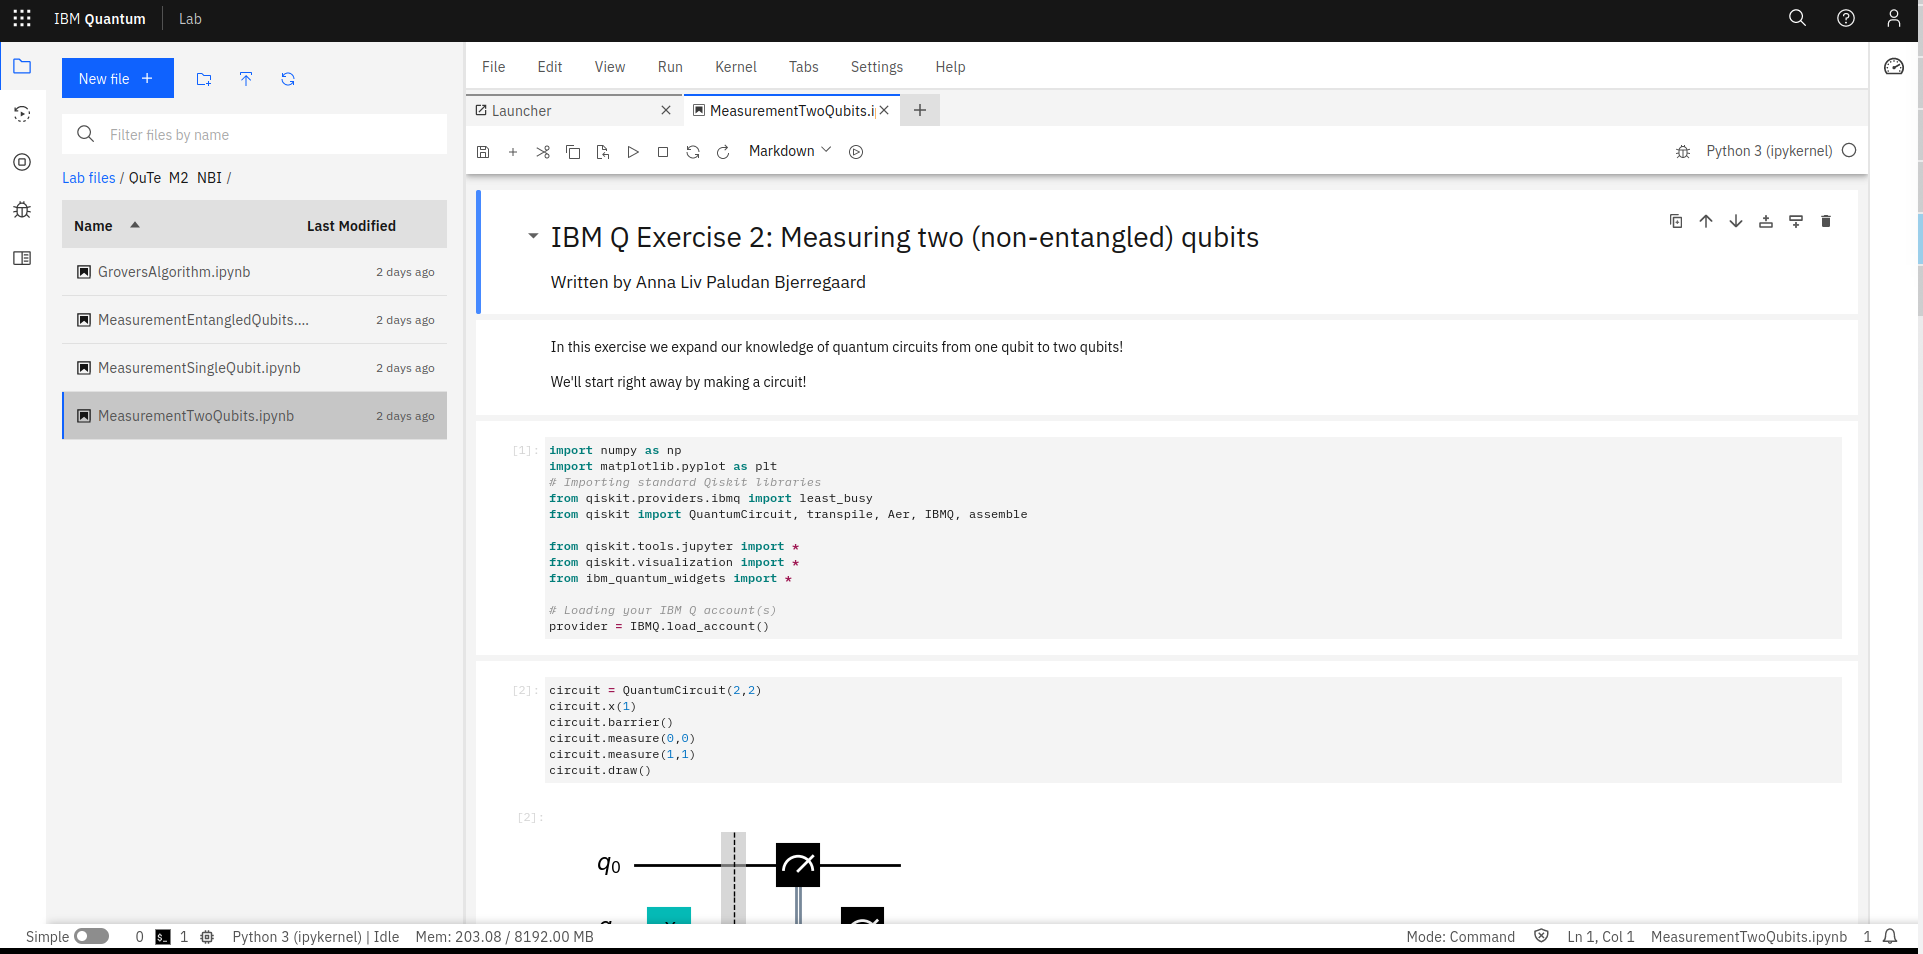
\includegraphics[width=9cm]{img/ibmq-two-qubit.png}
    \end{center}
\end{frame}

\begin{frame}
  \frametitle{Measurement of two (entangled) qubits}
While still at \href{https://lab.quantum-computing.ibm.com}{https://lab.quantum-computing.ibm.com} work on exercise \emph{MeasurementEntangledQubits.pynb}

  \begin{center}
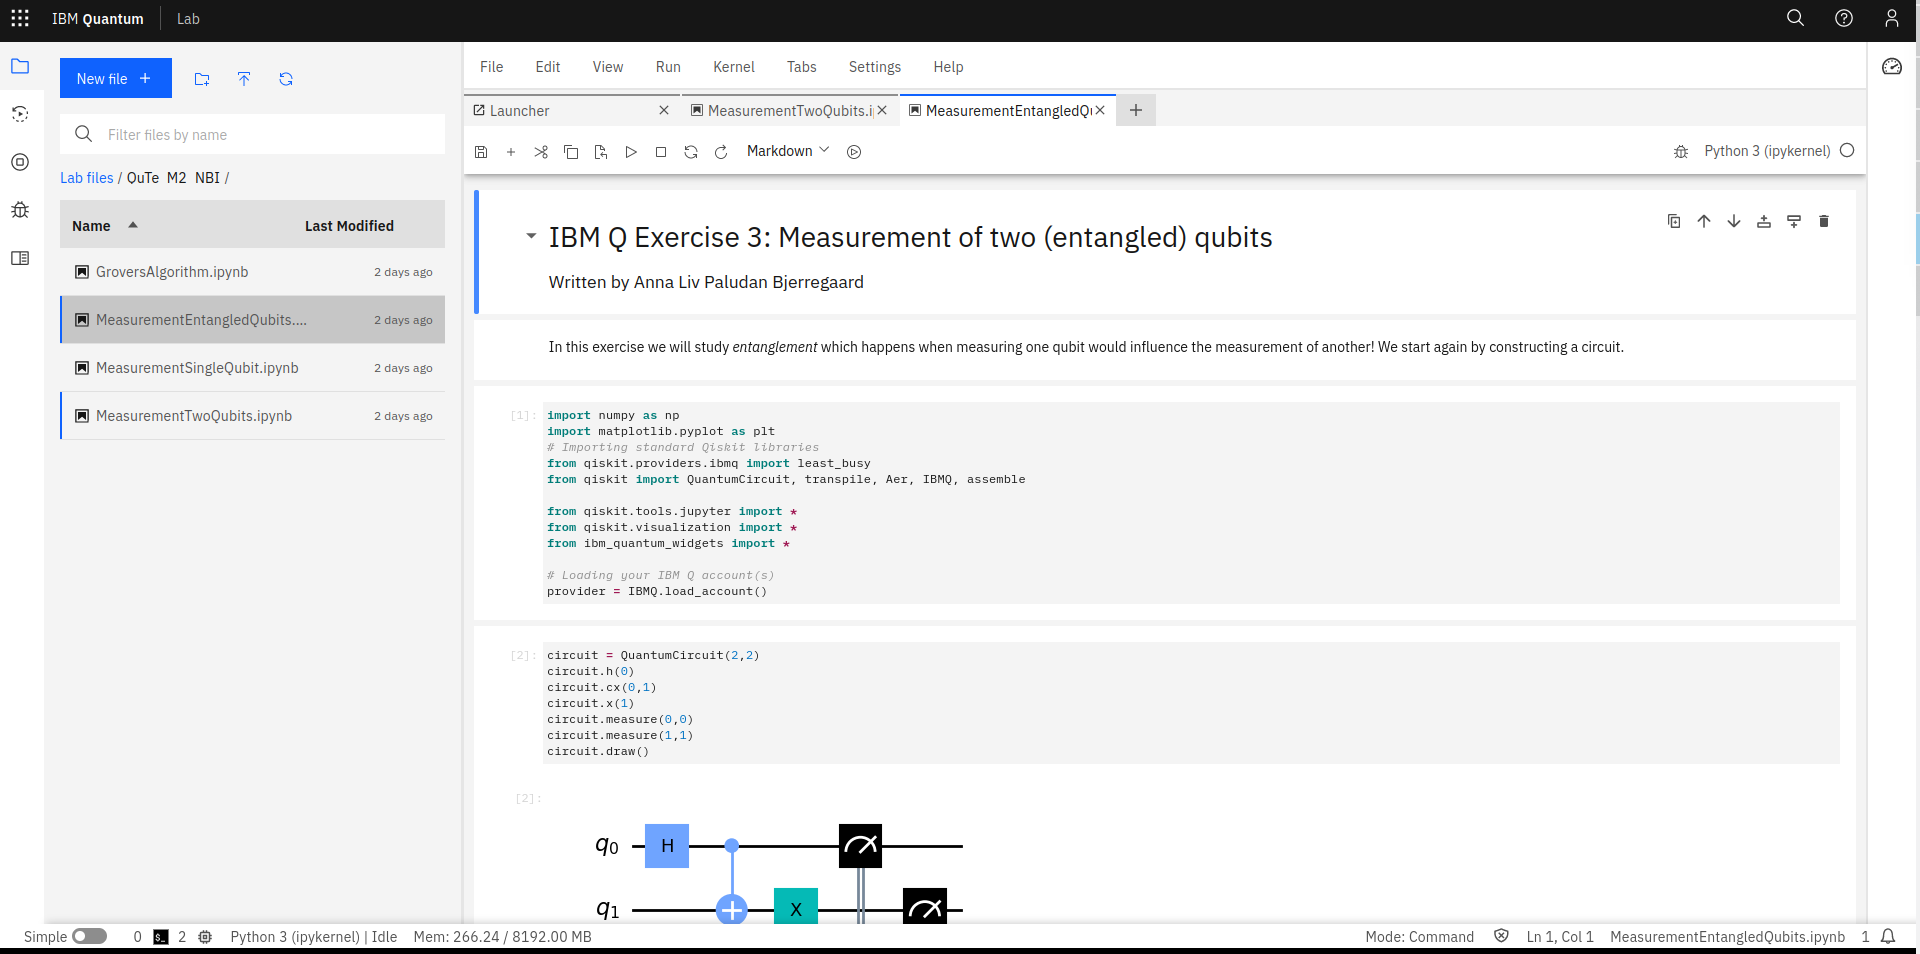
\includegraphics[width=9cm]{img/ibmq-entangled-qubits.png}
    \end{center}
\end{frame}

% \begin{frame}
%   \centering
%   
\includegraphics[width=7cm]{img/groovy-baby.jpeg}

%   \uncover<2>{\alert{NO, NO!}}
% \end{frame}

%   \begin{frame}
%     \section{\textbf{Grover} Baby! - Yeah!}
%     \centering
% 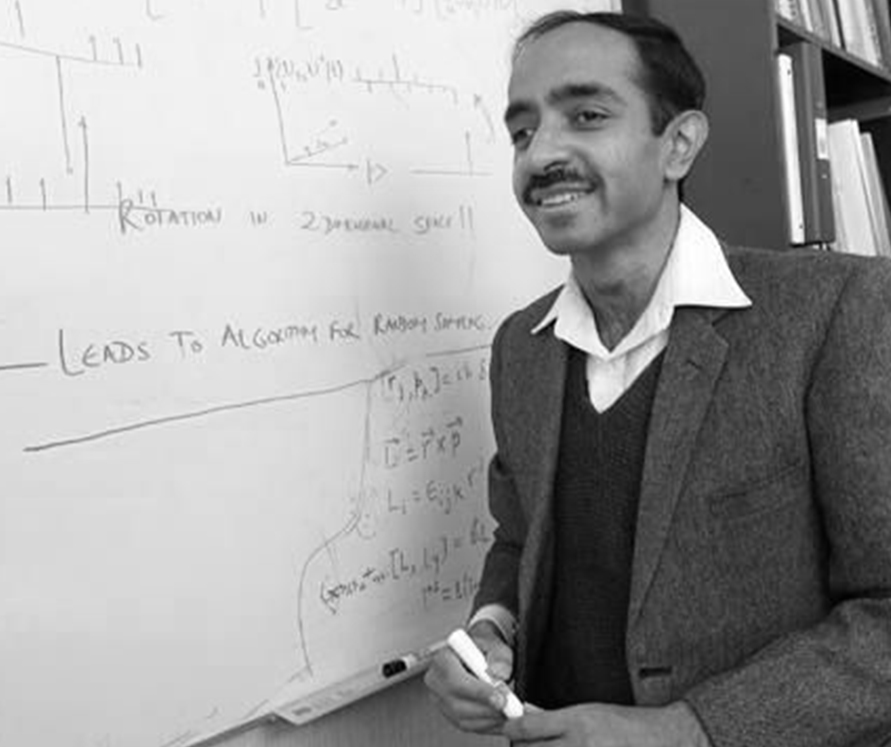
\includegraphics[width=5cm]{./img/Lov-Kumar-Grover.jpg}
%   \end{frame}
%   \begin{frame}
%     \frametitle{Grover's algorithm}
%     \begin{columns}
%       \begin{column}{0.6\linewidth}
%         \begin{itemize}
%         \item<+-> You have put your smartphone in the cabinet.
%         \item<+-> but you forgot the exact drawer!
%         \item<+-> A classical computer would on average use $\frac{N}{2}$ searches.
%         \item<+-> A quantum computer would on average use $\sqrt{N}$ searches using \emph{Grover's algorithm}.
%         \item<+-> Let us retrieve the phone using Grover's algorithm.
%         \end{itemize}
%       \end{column}
%       \begin{column}{0.4\linewidth}
%     \centering
% 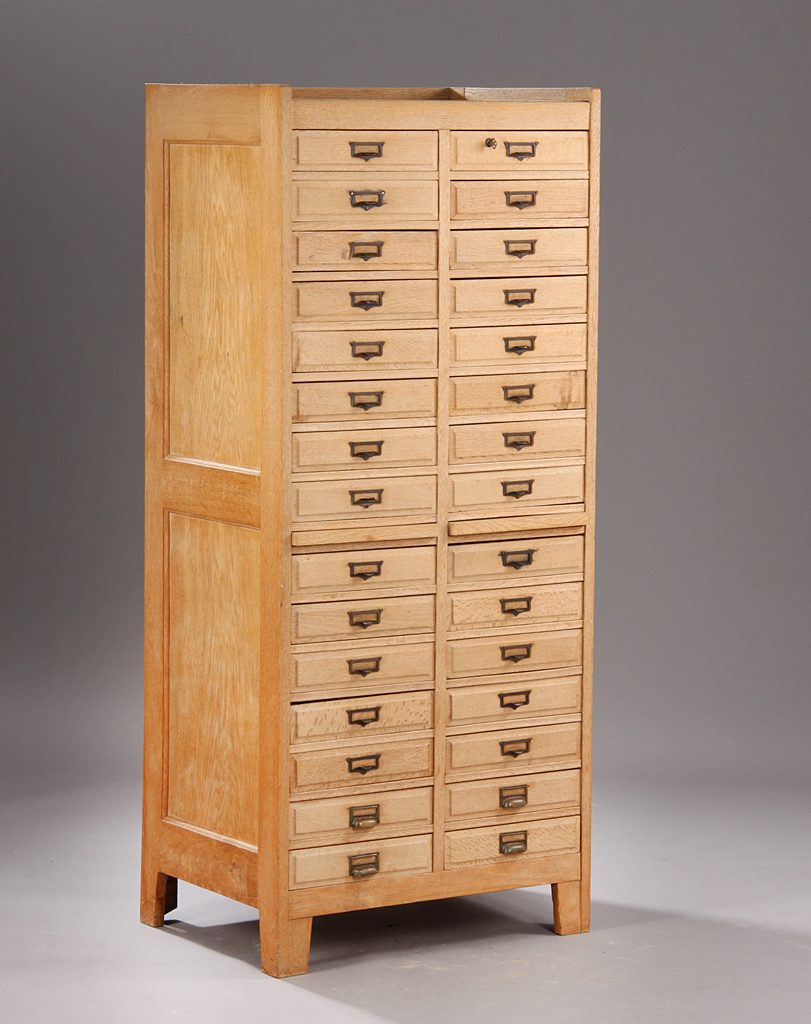
\includegraphics[width=0.8\linewidth]{./img/arkivskab.jpg}
%       \end{column}
%     \end{columns}
%   \end{frame}
%   \begin{frame}
%     \frametitle{Grover's algorithm with 4 drawers}
%     \begin{itemize}
%     \item 4 drawers can be represented by $n=2$ qubits in the special states $\ket{00}, \ket{01}, \ket{10}, \ket{11}$.
%     \item 00, 01, 10, 11 in binary are simply 0, 1, 2, 3 in decimal numbers \uncover<2->{\alert{if you recall.}}
%     \end{itemize}

%     \uncover<2->{
% \centering
%       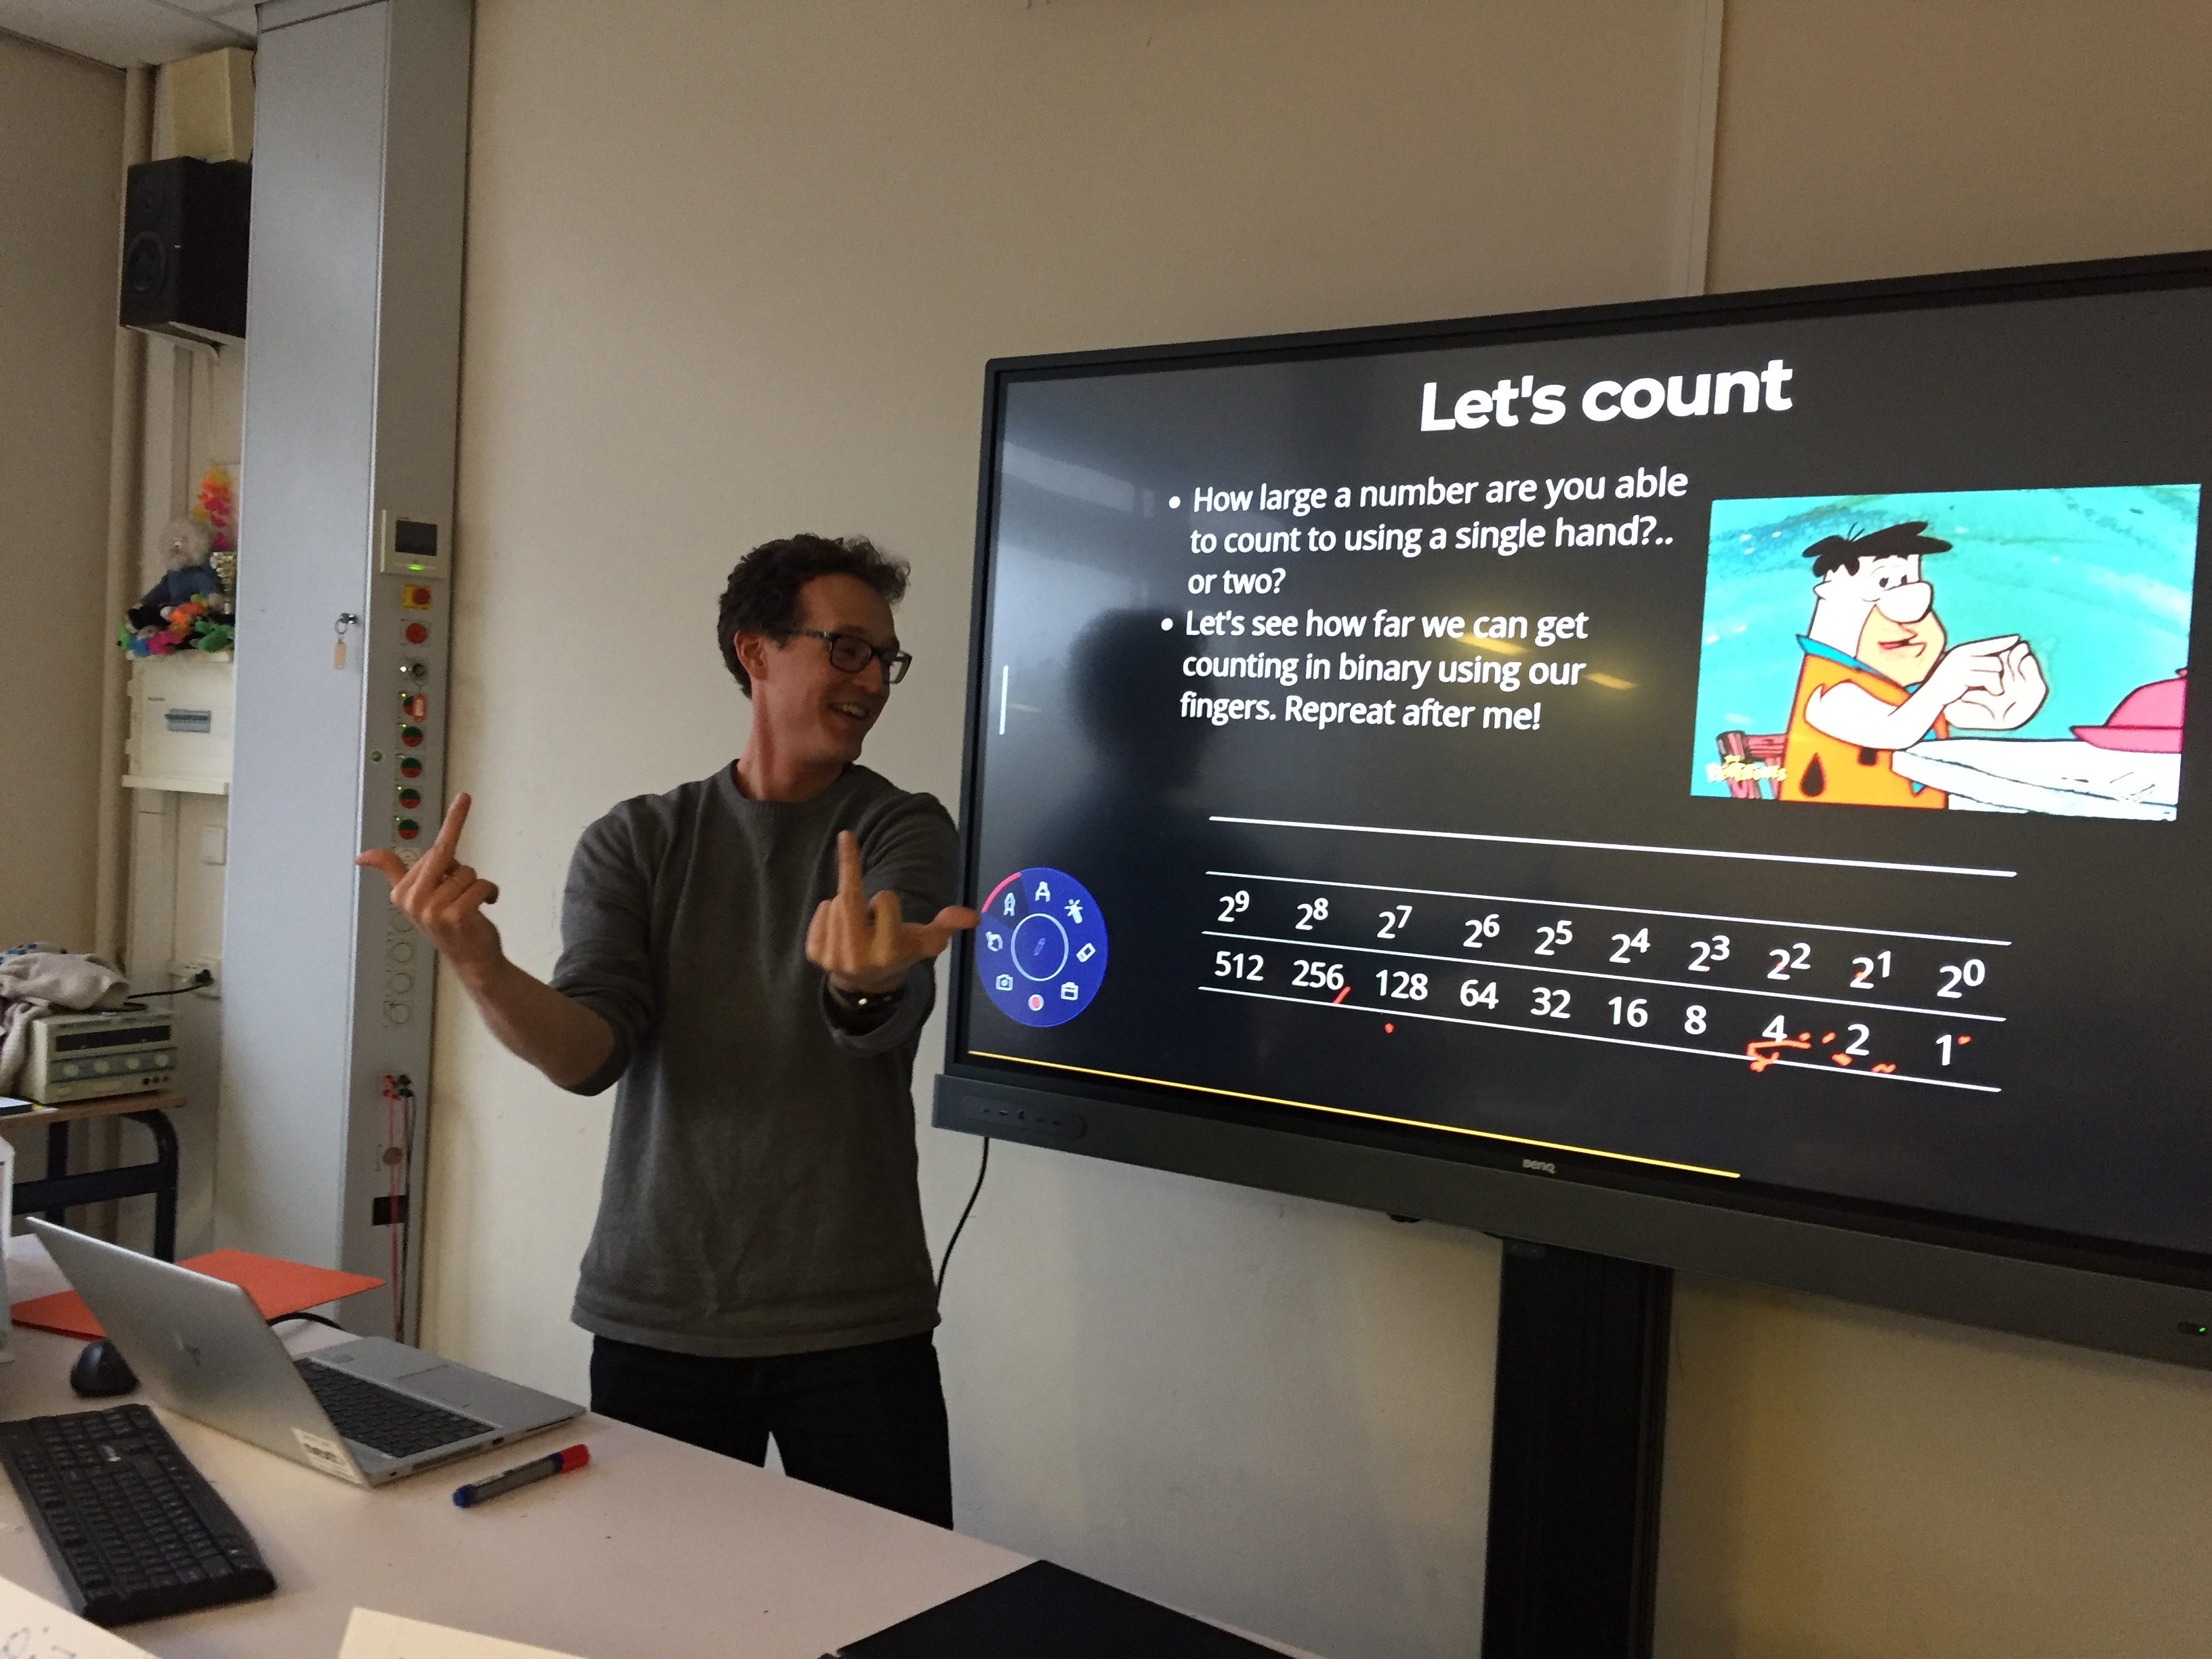
\includegraphics[width=6cm]{./img/tael_binaert_med_fingrene.jpg}}
%   \end{frame}
%   \begin{frame}
%     \frametitle{Grover's algorithm with 4 drawers}
%     \begin{itemize}
      
%     \item<1-> We assume that the phone is in drawer 11 (the 4th drawer labeled number 3 as we count from 0).
%     \item<2-> First step - Prepare the state: $\ket{\psi}=\frac{1}{2}\left( \ket{00}+\ket{01}+\ket{10}+\ket{11} \right)$.
%     \item<3-> Second step - act with the operator: $O = - \ket{11}\bra{11}$.
      
% \begin{align*}
%   O \ket{\psi} &= \left( -\ket{11}\bra{11} \right)\frac{1}{2}\left( \ket{00} + \ket{01}+\ket{10} + \ket{11} \right) \\
%   &=\frac{1}{2}\left( \ket{00} + \ket{01}+\ket{10} - \ket{11} \right)
% \end{align*}
%     \end{itemize}
%   \end{frame}
%   \begin{frame}
%     \frametitle{Grover's algorithm with 4 drawers}
%     \begin{itemize}
%     \item <1-> Third step - act with the operator: $\left( 2 \ket{\psi}\bra{\psi}- I \right)$.
      
%     \item<2-> The combined operator is called $G = \left( 2 \ket{\psi}\bra{\psi}-I \right) O$.
%     \item<3-> $G\ket{\psi}=\left( 2 \ket{\psi}\bra{\psi}-I \right) O\ket{\psi}$.
      
%     \item<4-> Fancy trick!
      
% \begin{align*}
%   O \ket{\psi} &= \frac{1}{2}\left( \ket{00}+\ket{01}+\ket{10}-\ket{11} \right) \\
%                &=\frac{1}{2}\left( \ket{00}+\ket{01}+\ket{10}+\ket{11} \right) - \ket{11} \\
%   &= \ket{\psi} - \ket{11}
% \end{align*}
      
%     \end{itemize}
%   \end{frame}
%   \begin{frame}
%     \frametitle{Grover's algorithm with 4 drawers}
%     \begin{itemize}
%     \item<1-> All combined:
      
% \begin{align*}
%   G\ket{\psi}&=\left( 2 \ket{\psi}\bra{\psi}-I \right) O\ket{\psi} \\
%              &=\left( 2 \ket{\psi}\bra{\psi}-I \right) \left( \ket{\psi} - \ket{11} \right) \\
%              &=2 \ket{\psi}\braket{\psi|\psi} - I \ket{\psi} - 2 \ket{\psi}\braket{\psi|11} + I \ket{11} \\
%              &=2 \ket{\psi} - \ket{\psi} - 2 \ket{\psi}\frac{1}{2} + \ket{11} \\
%   &= \ket{11}
% \end{align*}
% \item<2-> If we measure now we will get 11 with 100\% probability.
% \item<3-|alert@3> But it's like cheating! We told the \emph{Oracle} (O operator) where the phone was from the beginning.
% \item<4-|alert@4> Grover's algorithm needs to be part of a complete algorithm.
%     \end{itemize}
%   \end{frame}
%   \begin{frame}
%     \frametitle{Grover's algorithm with 8 drawers}
%     Read the example about Grover's algorithm for $N=8$ on page 22 and 23 in the notes.
%   \end{frame}

%   \begin{frame}
%     \frametitle{Grover's algorithm on IBM Q}
%     Now finally open and work on the exercise \emph{GroversAlgorithm.ipynb} on \href{https://lab.quantum-computing.ibm.com}{https://lab.quantum-computing.ibm.com}

%     \begin{center}
%       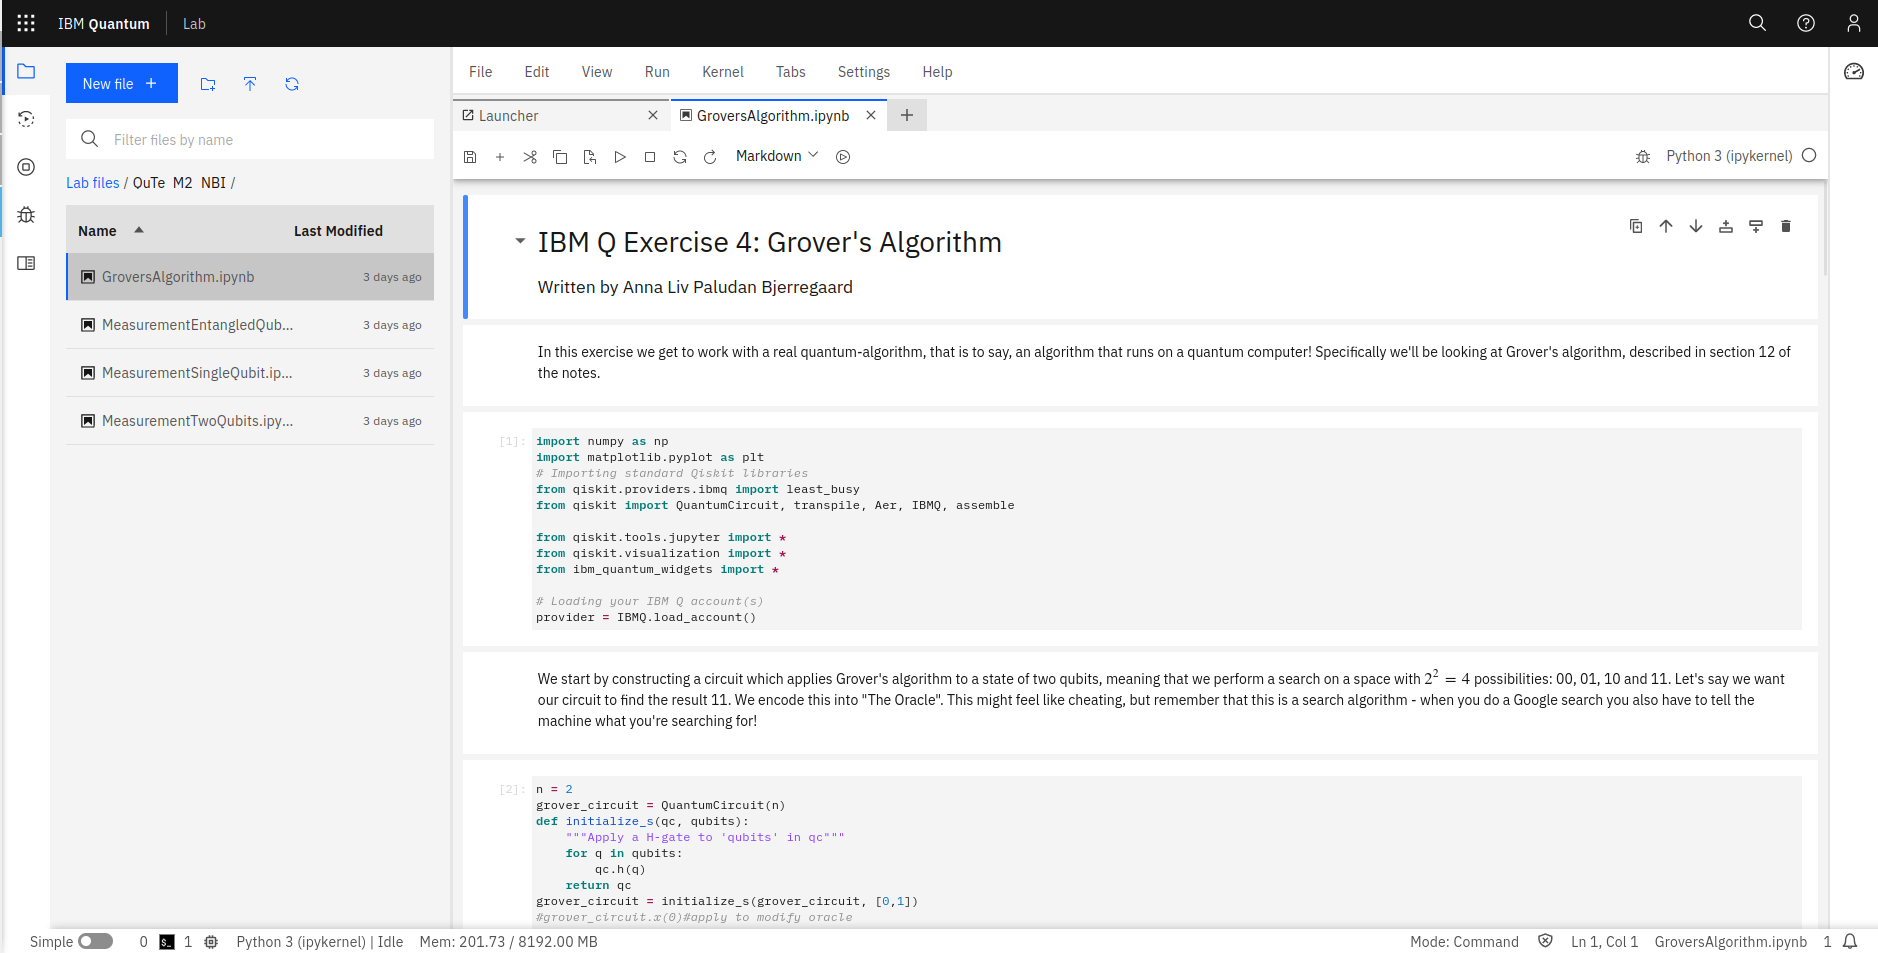
\includegraphics[width=10cm]{./img/ibm-q-grover.png}
%       \end{center}
%   \end{frame}
\end{document}